\begin{figure}[htbp]
	\centering
    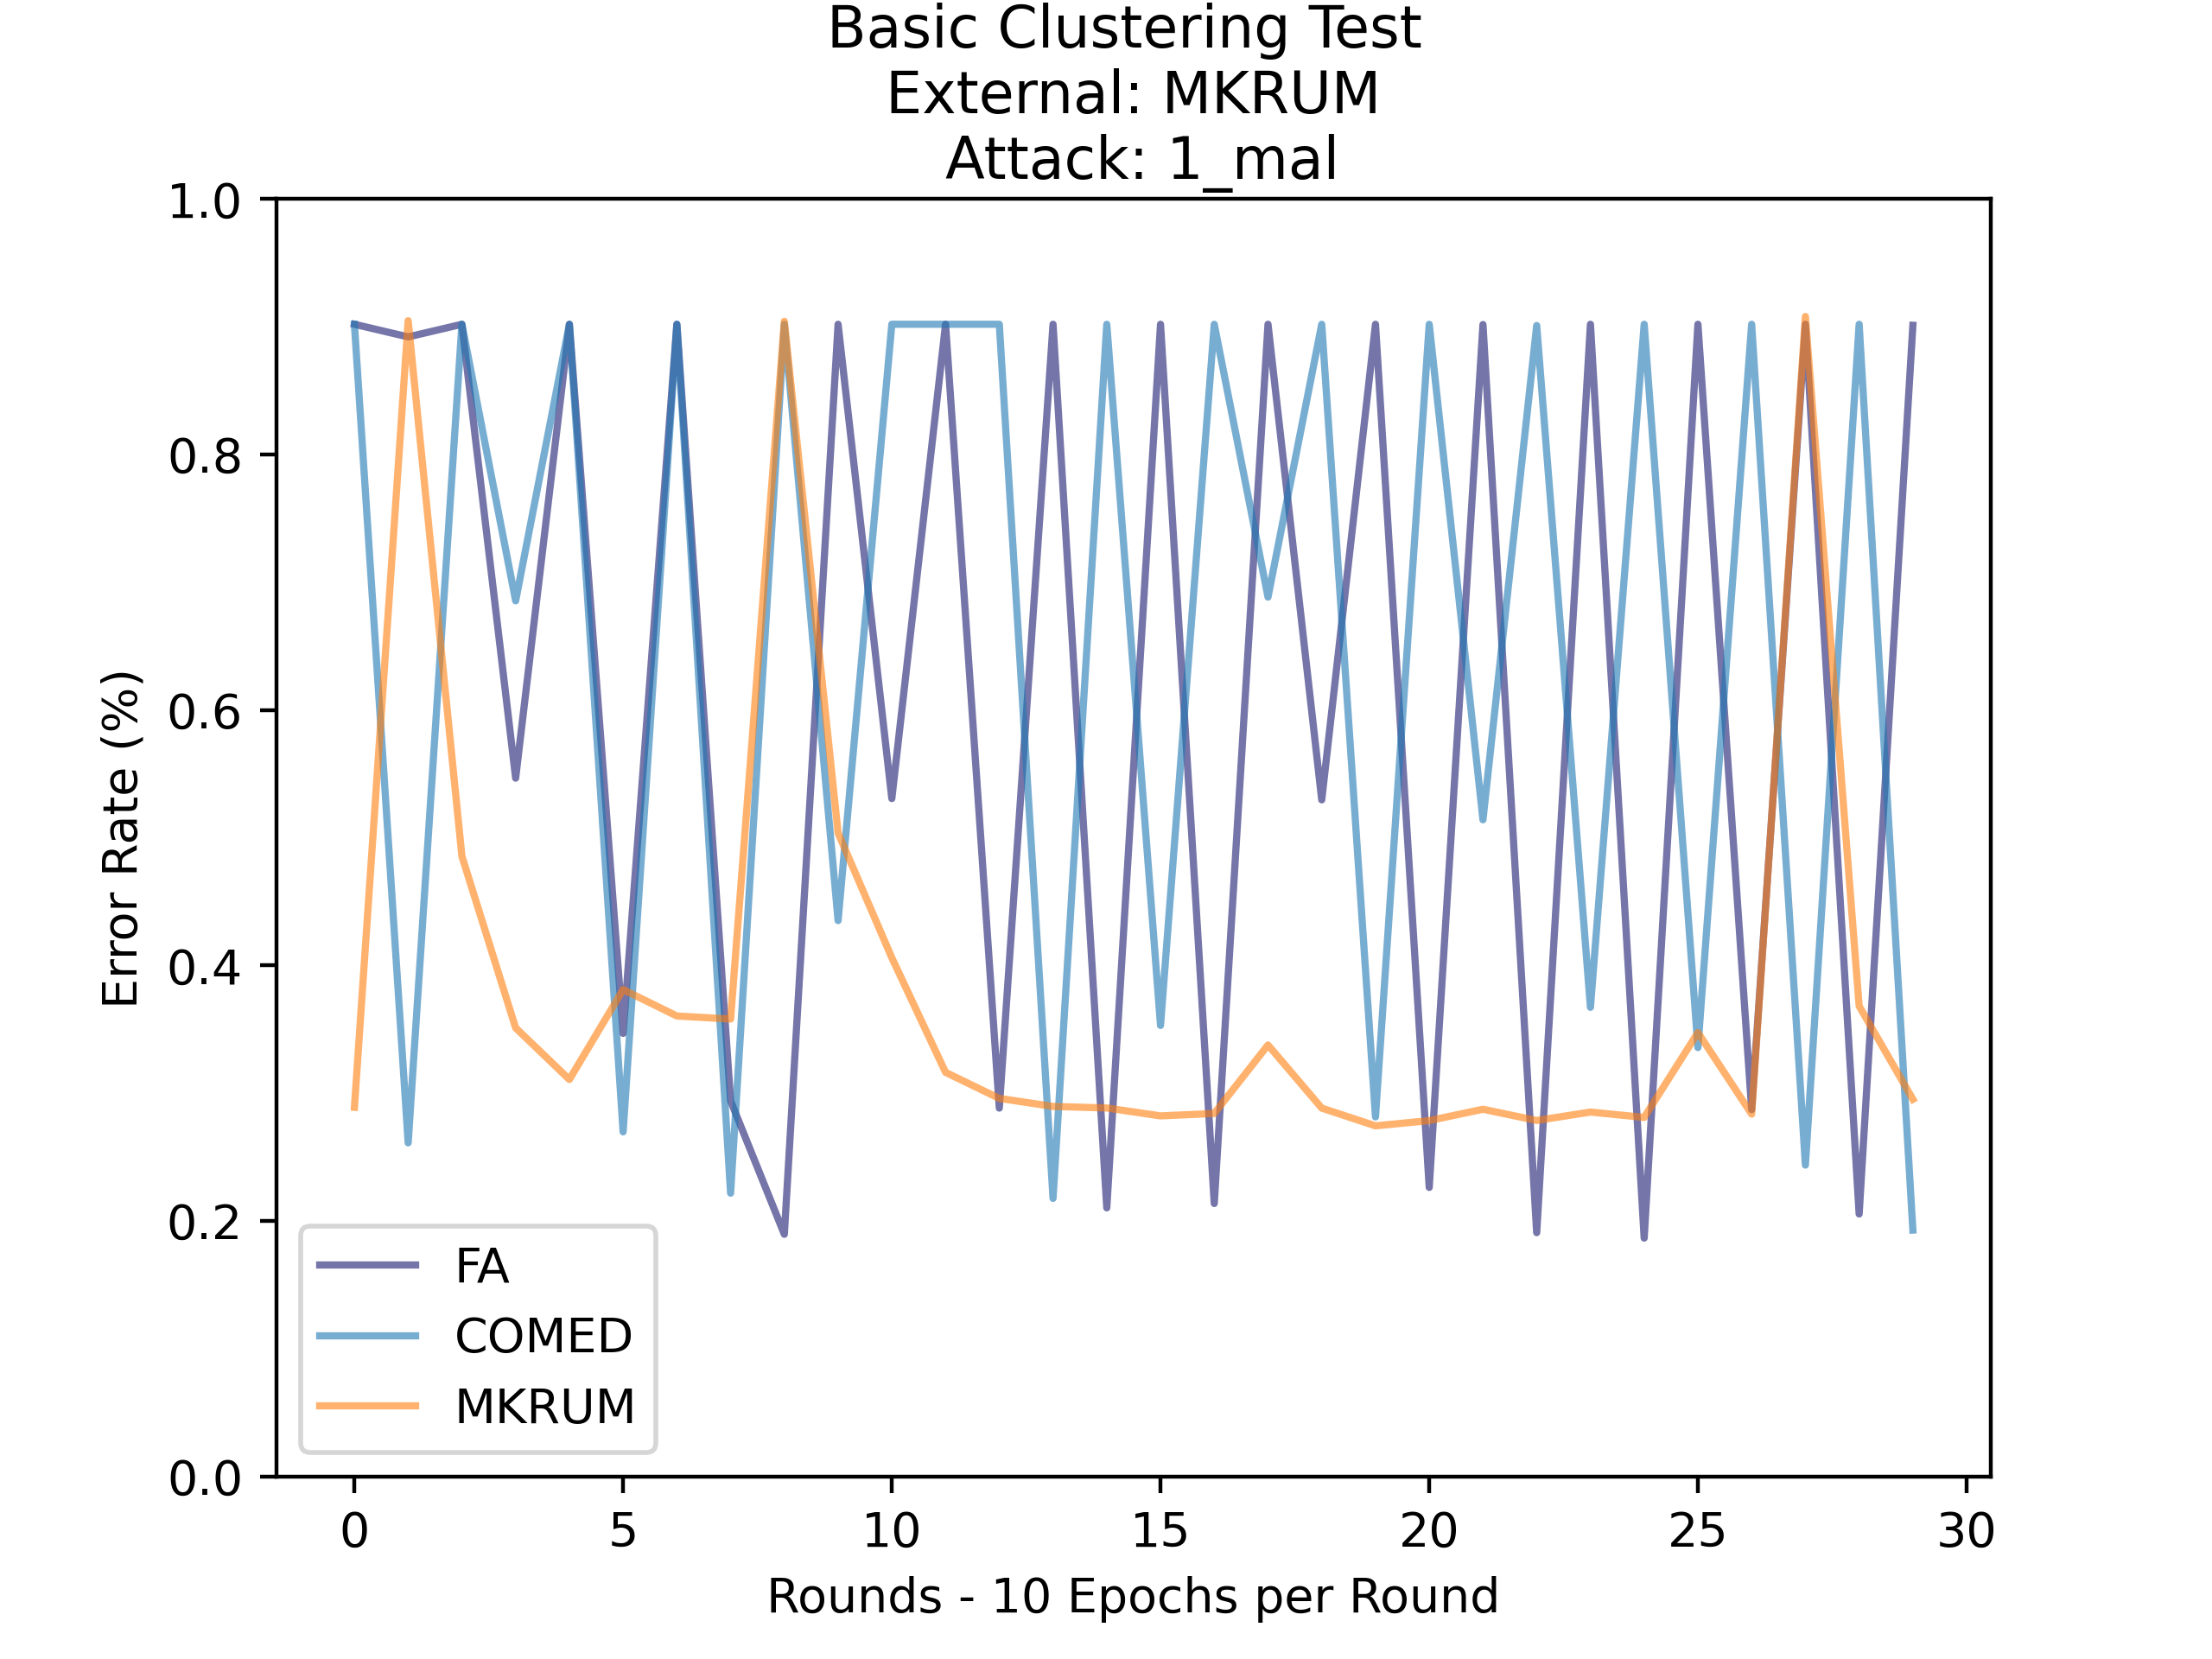
\includegraphics[scale=0.5]{my_agg/graphs/cluster_mkrum_1.png}
	\caption{Error Rate of K-Means Clustering when MKRUM is the External Aggregator}
	\label{fig:mkrum_bad}
\end{figure}

\begin{figure}[htbp]
	\centering
    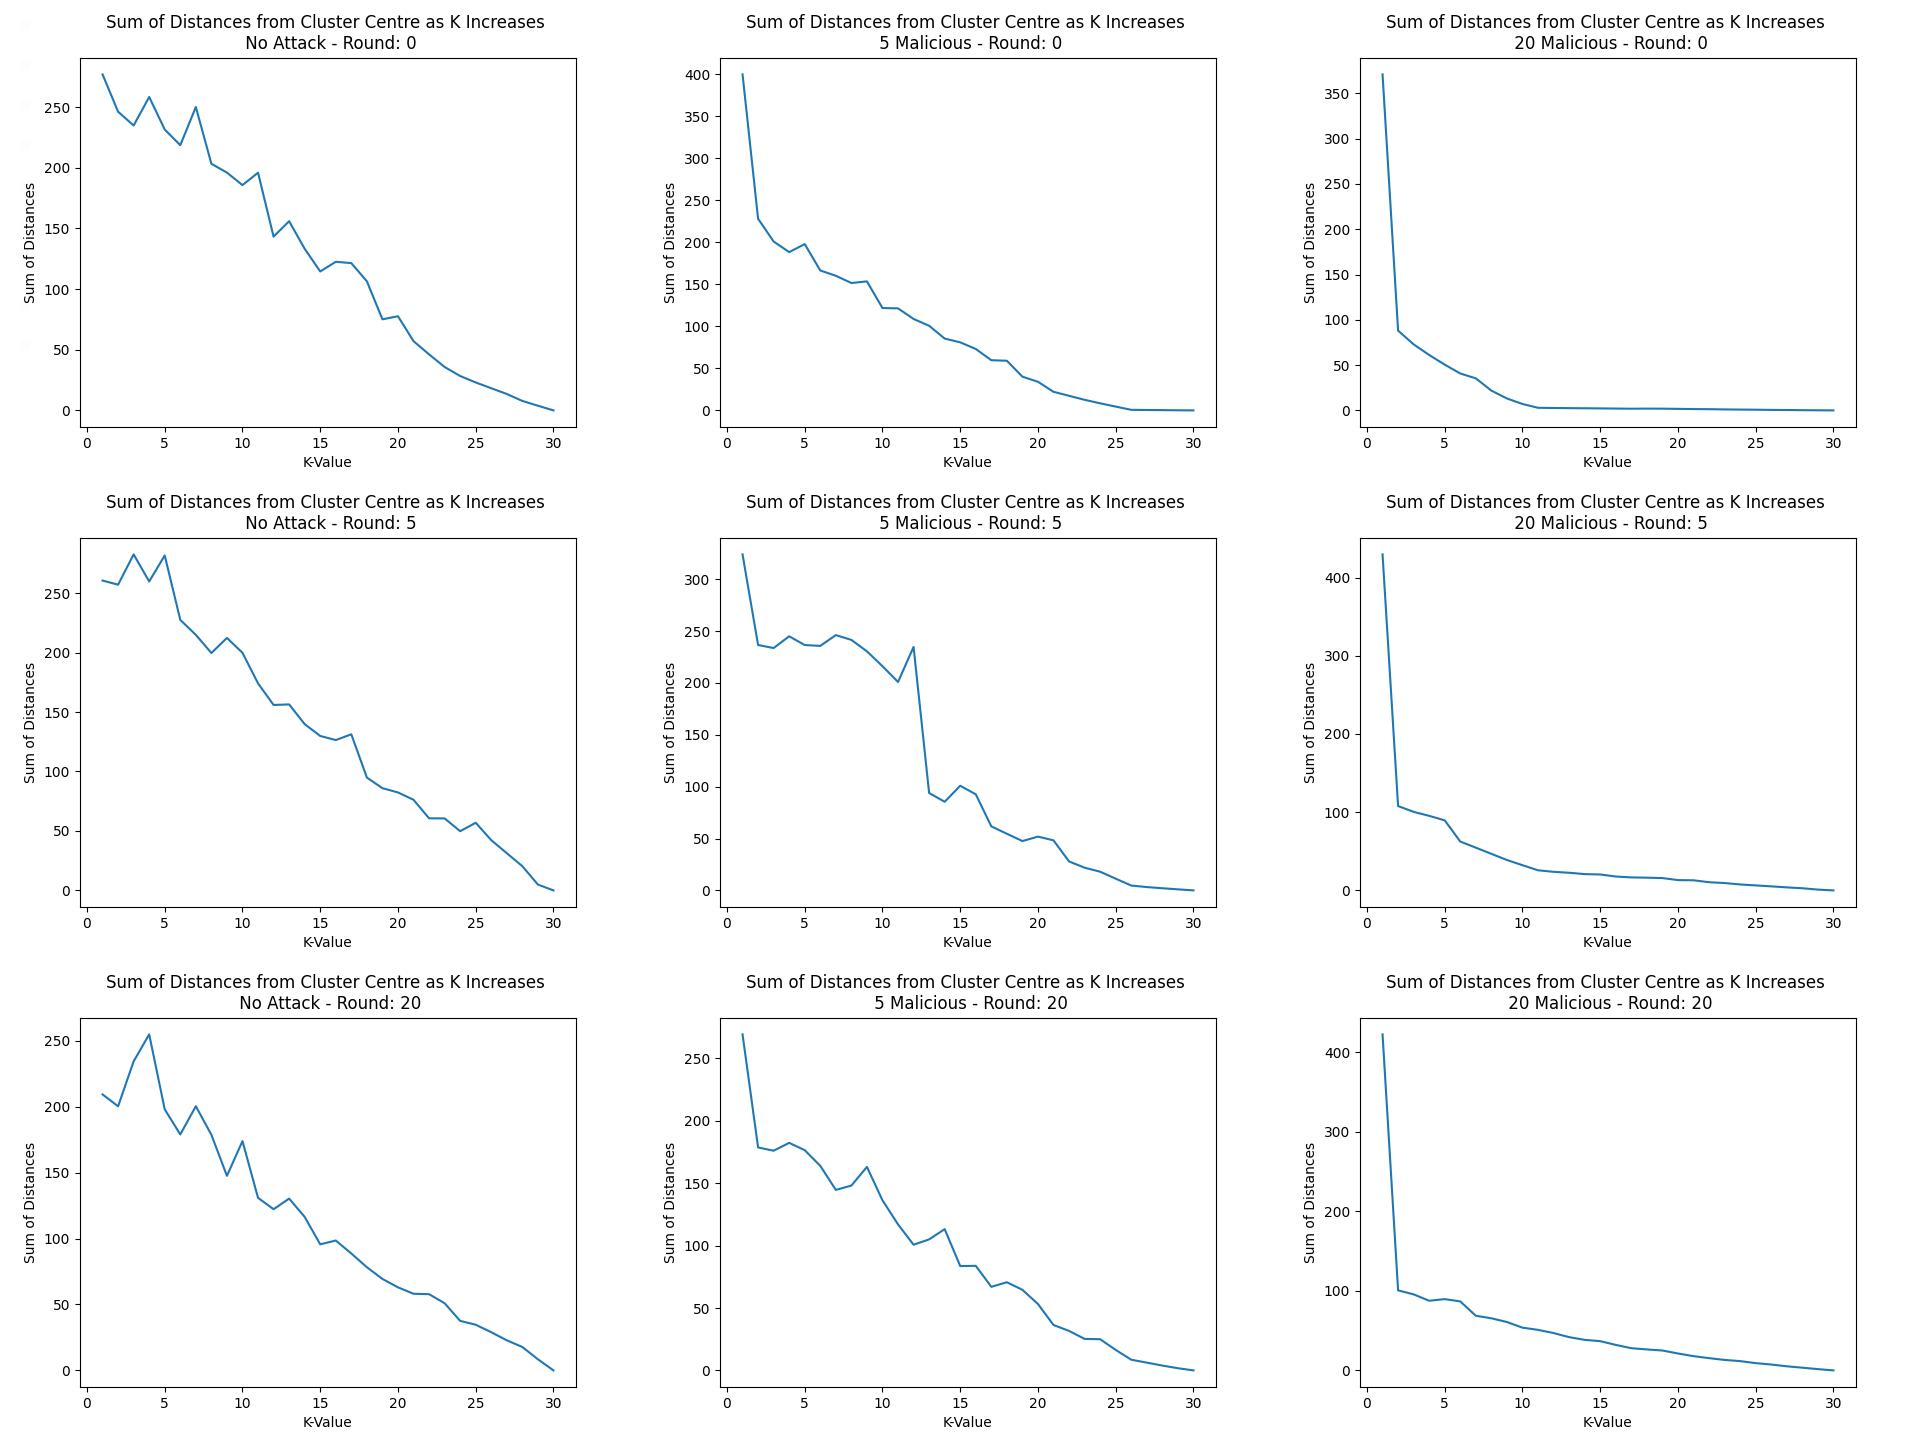
\includegraphics[scale=0.25]{my_agg/graphs/k_elbow.png}
	\caption{Finding the Elbow Point for K-Means Clustering}
	\label{fig:k_elbow}
\end{figure}

\begin{figure}[htbp]
	\centering
    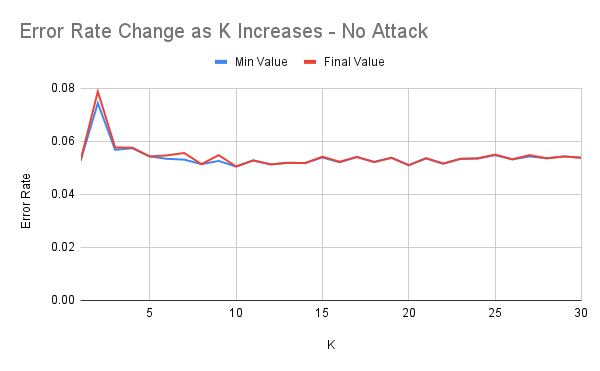
\includegraphics[scale=0.5]{my_agg/graphs/k_elbow_0.png}
	\caption{Error Rate As K Increases - No Attack}
	\label{fig:k_elbow_0}
\end{figure}

\begin{figure}[htbp]
	\centering
    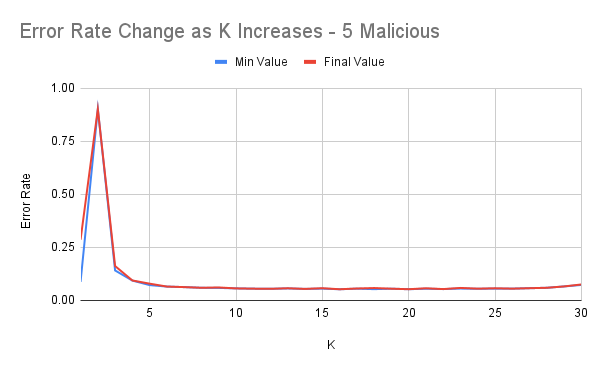
\includegraphics[scale=0.5]{my_agg/graphs/k_elbow_5.png}
	\caption{Error Rate As K Increases - 5 Malicious}
	\label{fig:k_elbow_5}
\end{figure}

\begin{figure}[htbp]
	\centering
    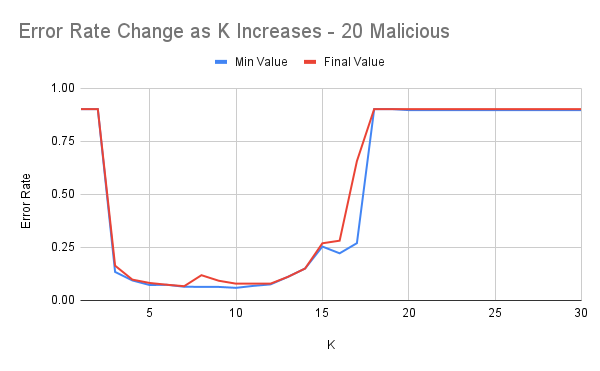
\includegraphics[scale=0.5]{my_agg/graphs/k_elbow_20.png}
	\caption{Error Rate As K Increases - 20 Malicious}
	\label{fig:k_elbow_20}
\end{figure}

\begin{figure}[htbp]
	\centering
    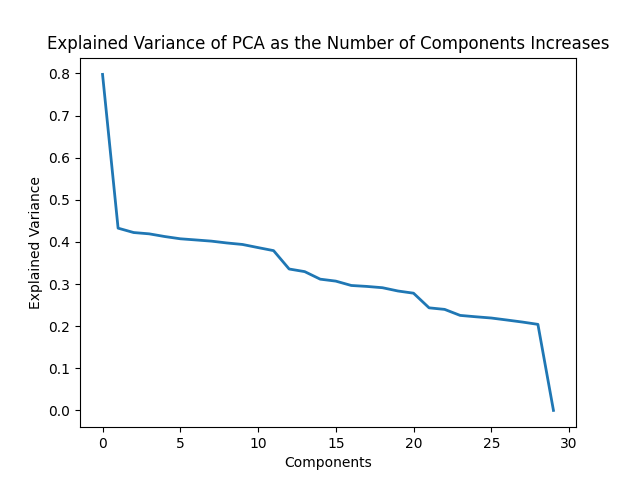
\includegraphics[scale=0.5]{my_agg/graphs/0_r1.png}
	\caption{Explained Variance with No Attacks at Round 1}
	\label{fig:pca_01}
\end{figure}

\begin{figure}[htbp]
	\centering
    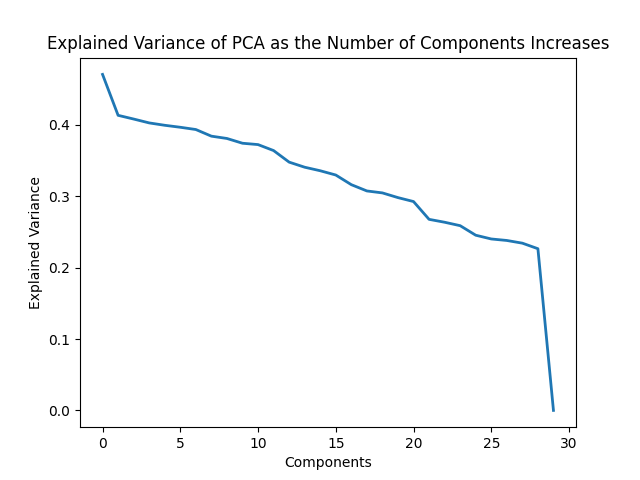
\includegraphics[scale=0.5]{my_agg/graphs/0_r2.png}
	\caption{Explained Variance with No Attacks at Round 2}
	\label{fig:pca_02}
\end{figure}

\begin{figure}[htbp]
	\centering
    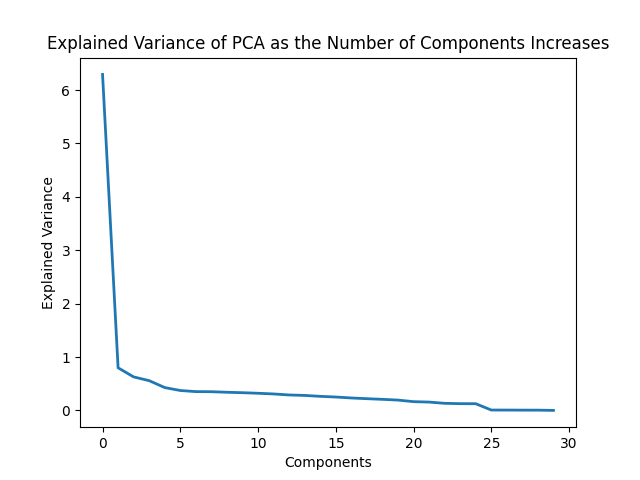
\includegraphics[scale=0.5]{my_agg/graphs/5_r0.png}
	\caption{Explained Variance with 5 Malicious at Round 0}
	\label{fig:pca_50}
\end{figure}

\begin{figure}[htbp]
	\centering
    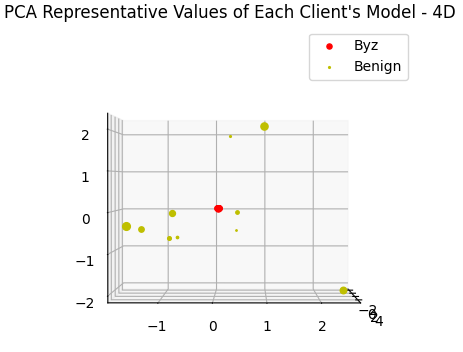
\includegraphics[scale=0.6]{my_agg/graphs/4d_diff.png}
	\caption{PCA Transform Positions in 4D, Alternate View - 20 Malicious - Round 0}
	\label{fig:4d_diff}
\end{figure}

\begin{figure}[htbp]
	\centering
    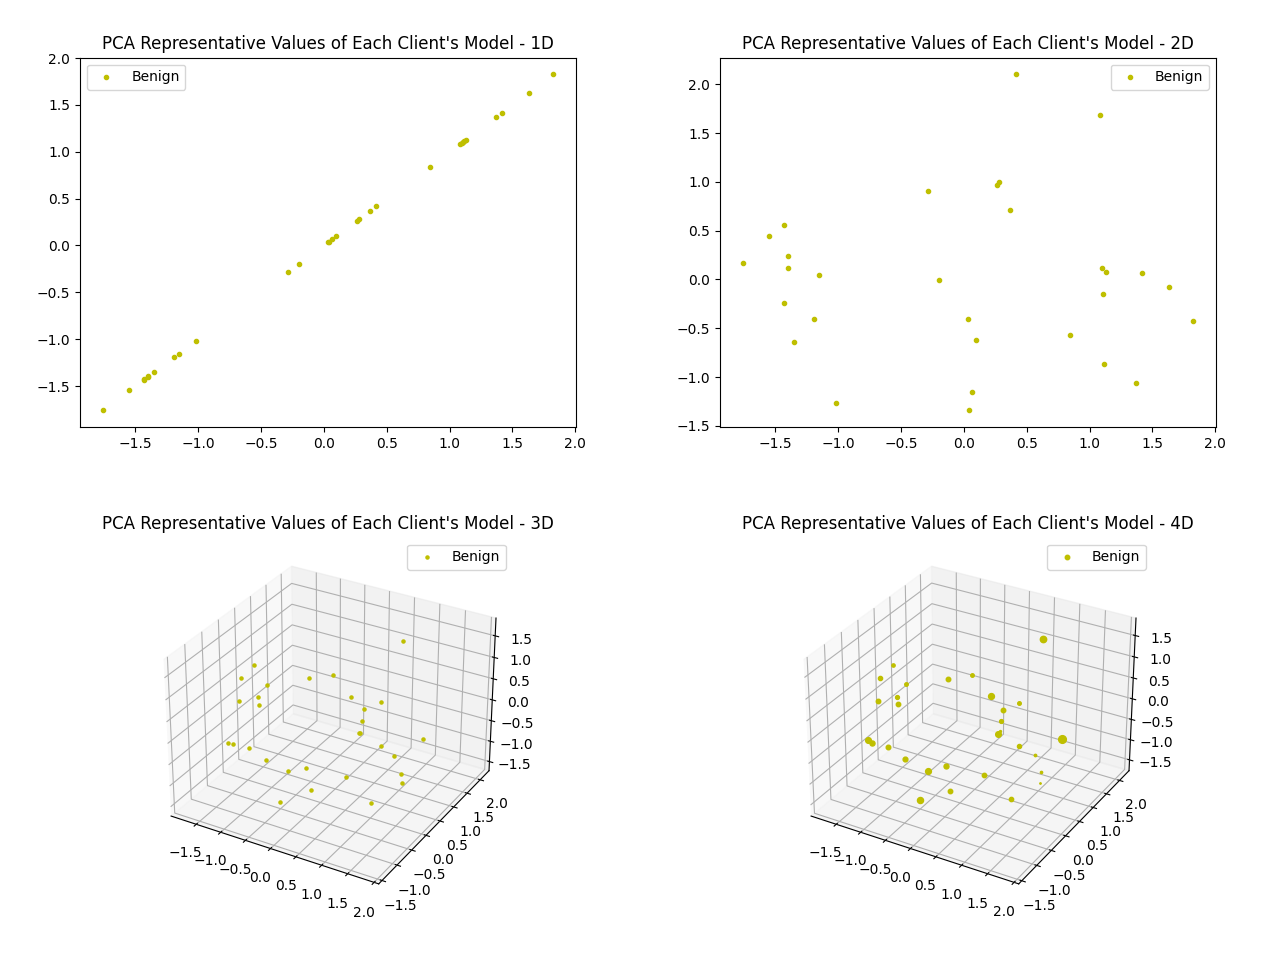
\includegraphics[scale=0.3]{my_agg/graphs/0mal_dims.png}
	\caption{PCA Transform Positions over Four Dimensions - No Attacks - Round 0}
	\label{fig:0mal_dims}
\end{figure}

\begin{figure}[htbp]
	\centering
    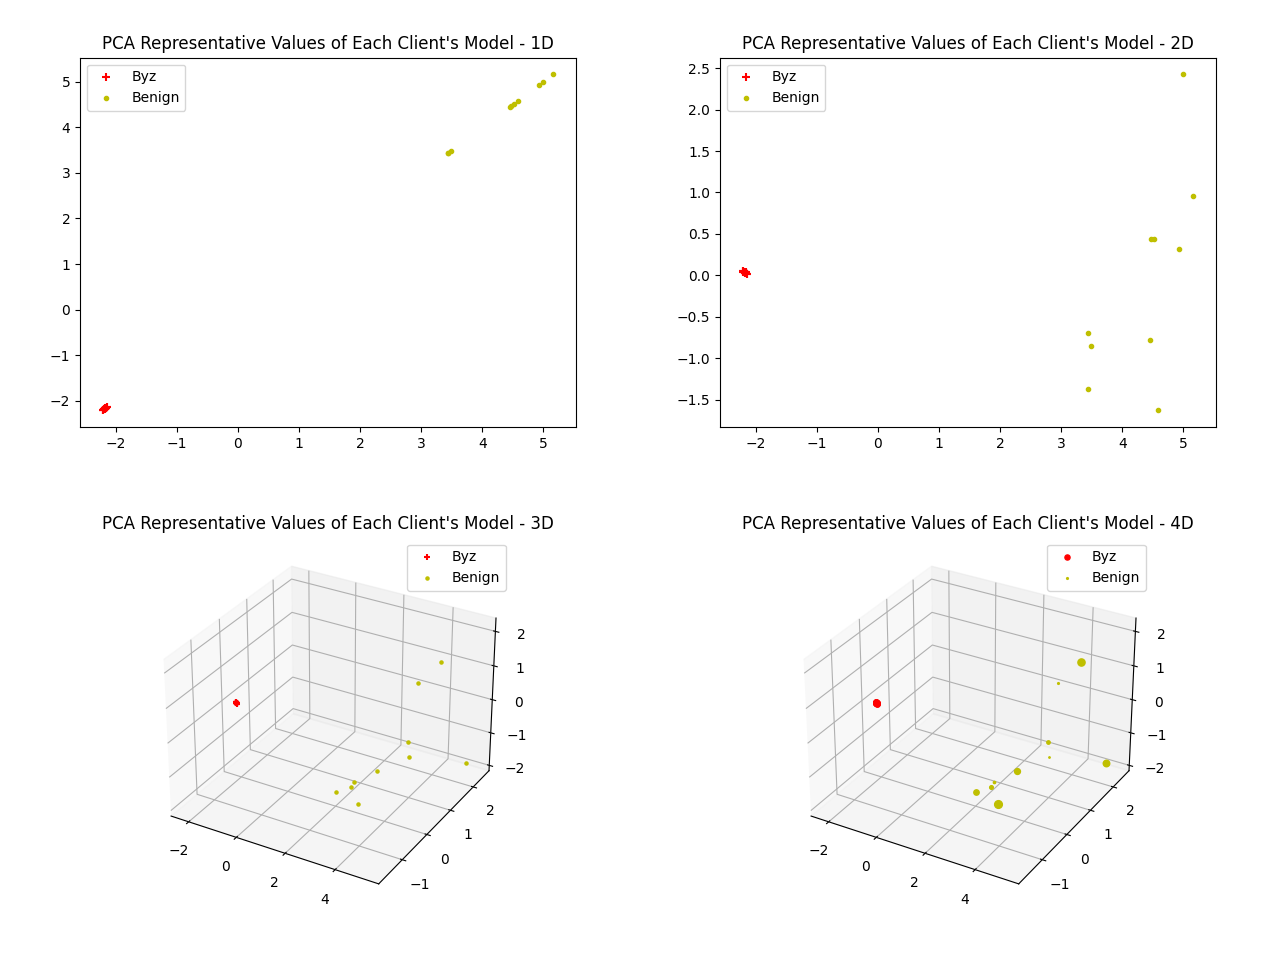
\includegraphics[scale=0.3]{my_agg/graphs/20mal_dims.png}
	\caption{PCA Transform Positions over Four Dimensions - 20 Malicious - Round 0}
	\label{fig:20mal_dims}
\end{figure}

\begin{figure}[htbp]
	\centering
    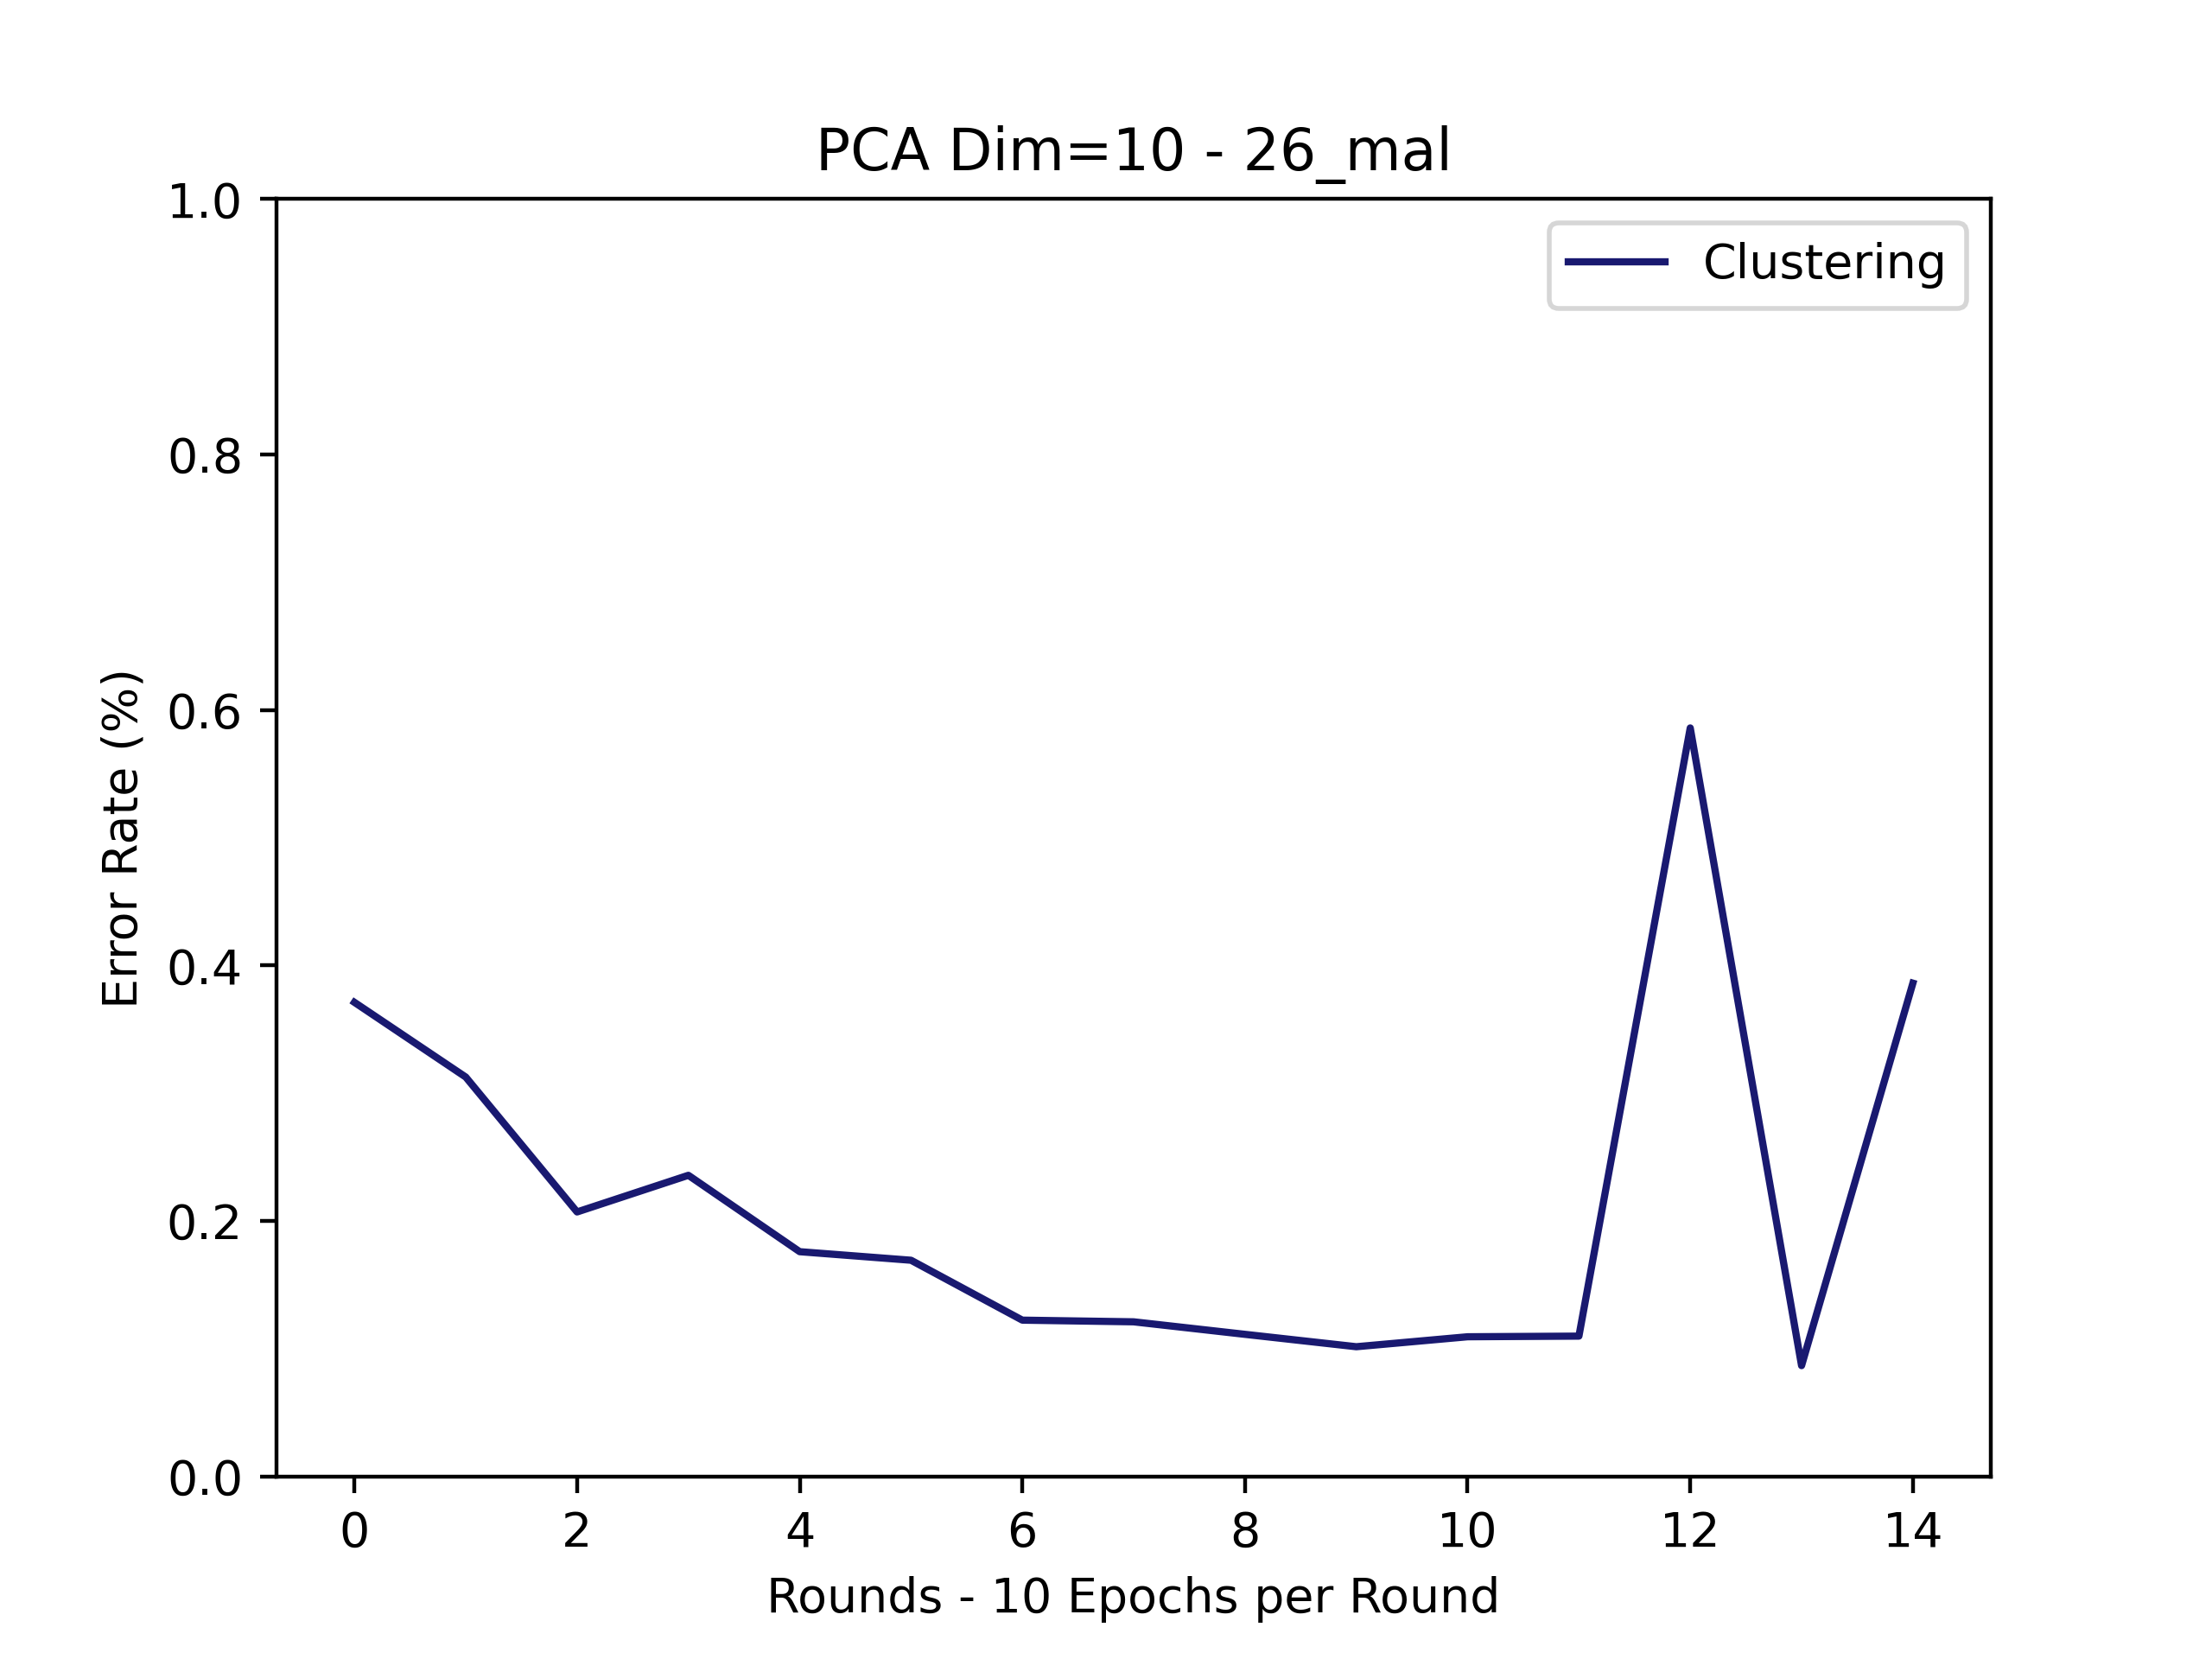
\includegraphics[scale=0.5]{my_agg/graphs/dim10_26mal.png}
	\caption{Less Smooth Performance Exhibited when Dim=10 with 26 Malicious}
	\label{fig:dim10_26mal}
\end{figure}

\begin{figure}[htbp]
	\centering
    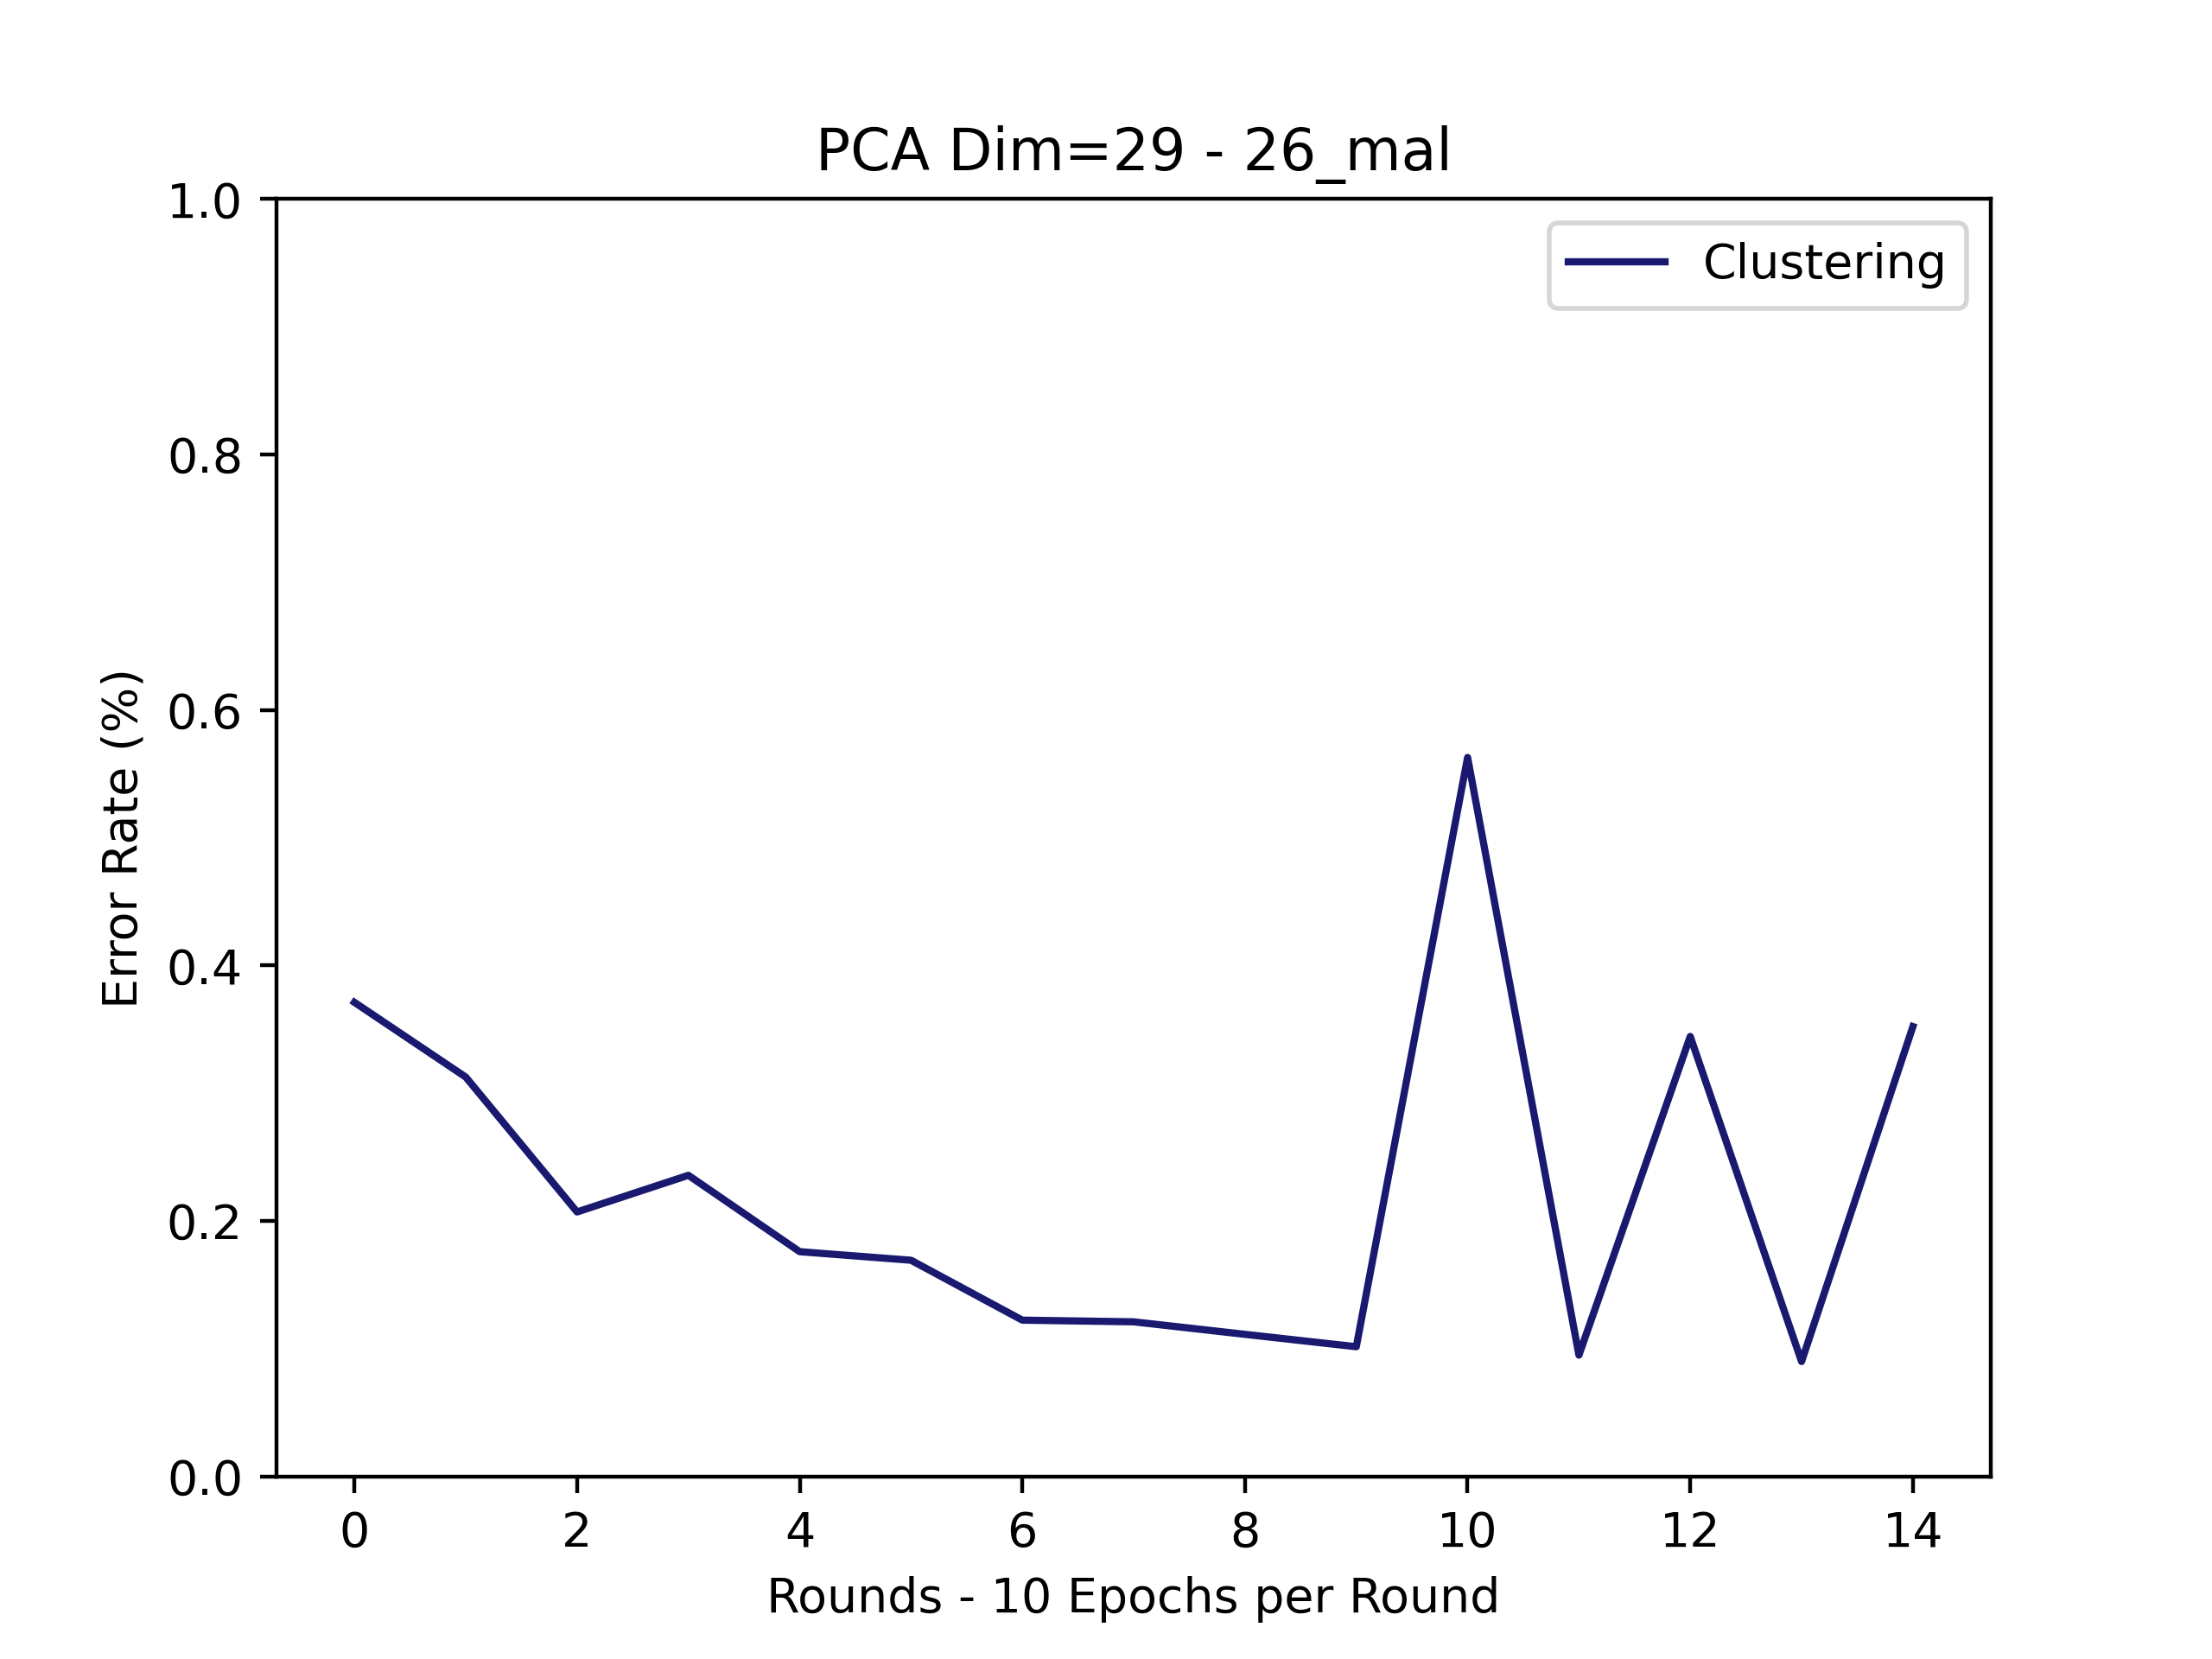
\includegraphics[scale=0.5]{my_agg/graphs/dim29_26mal.png}
	\caption{Less Smooth Performance Exhibited when Dim=29 with 26 Malicious}
	\label{fig:dim29_26mal}
\end{figure}

\begin{figure}[htbp]
	\centering
    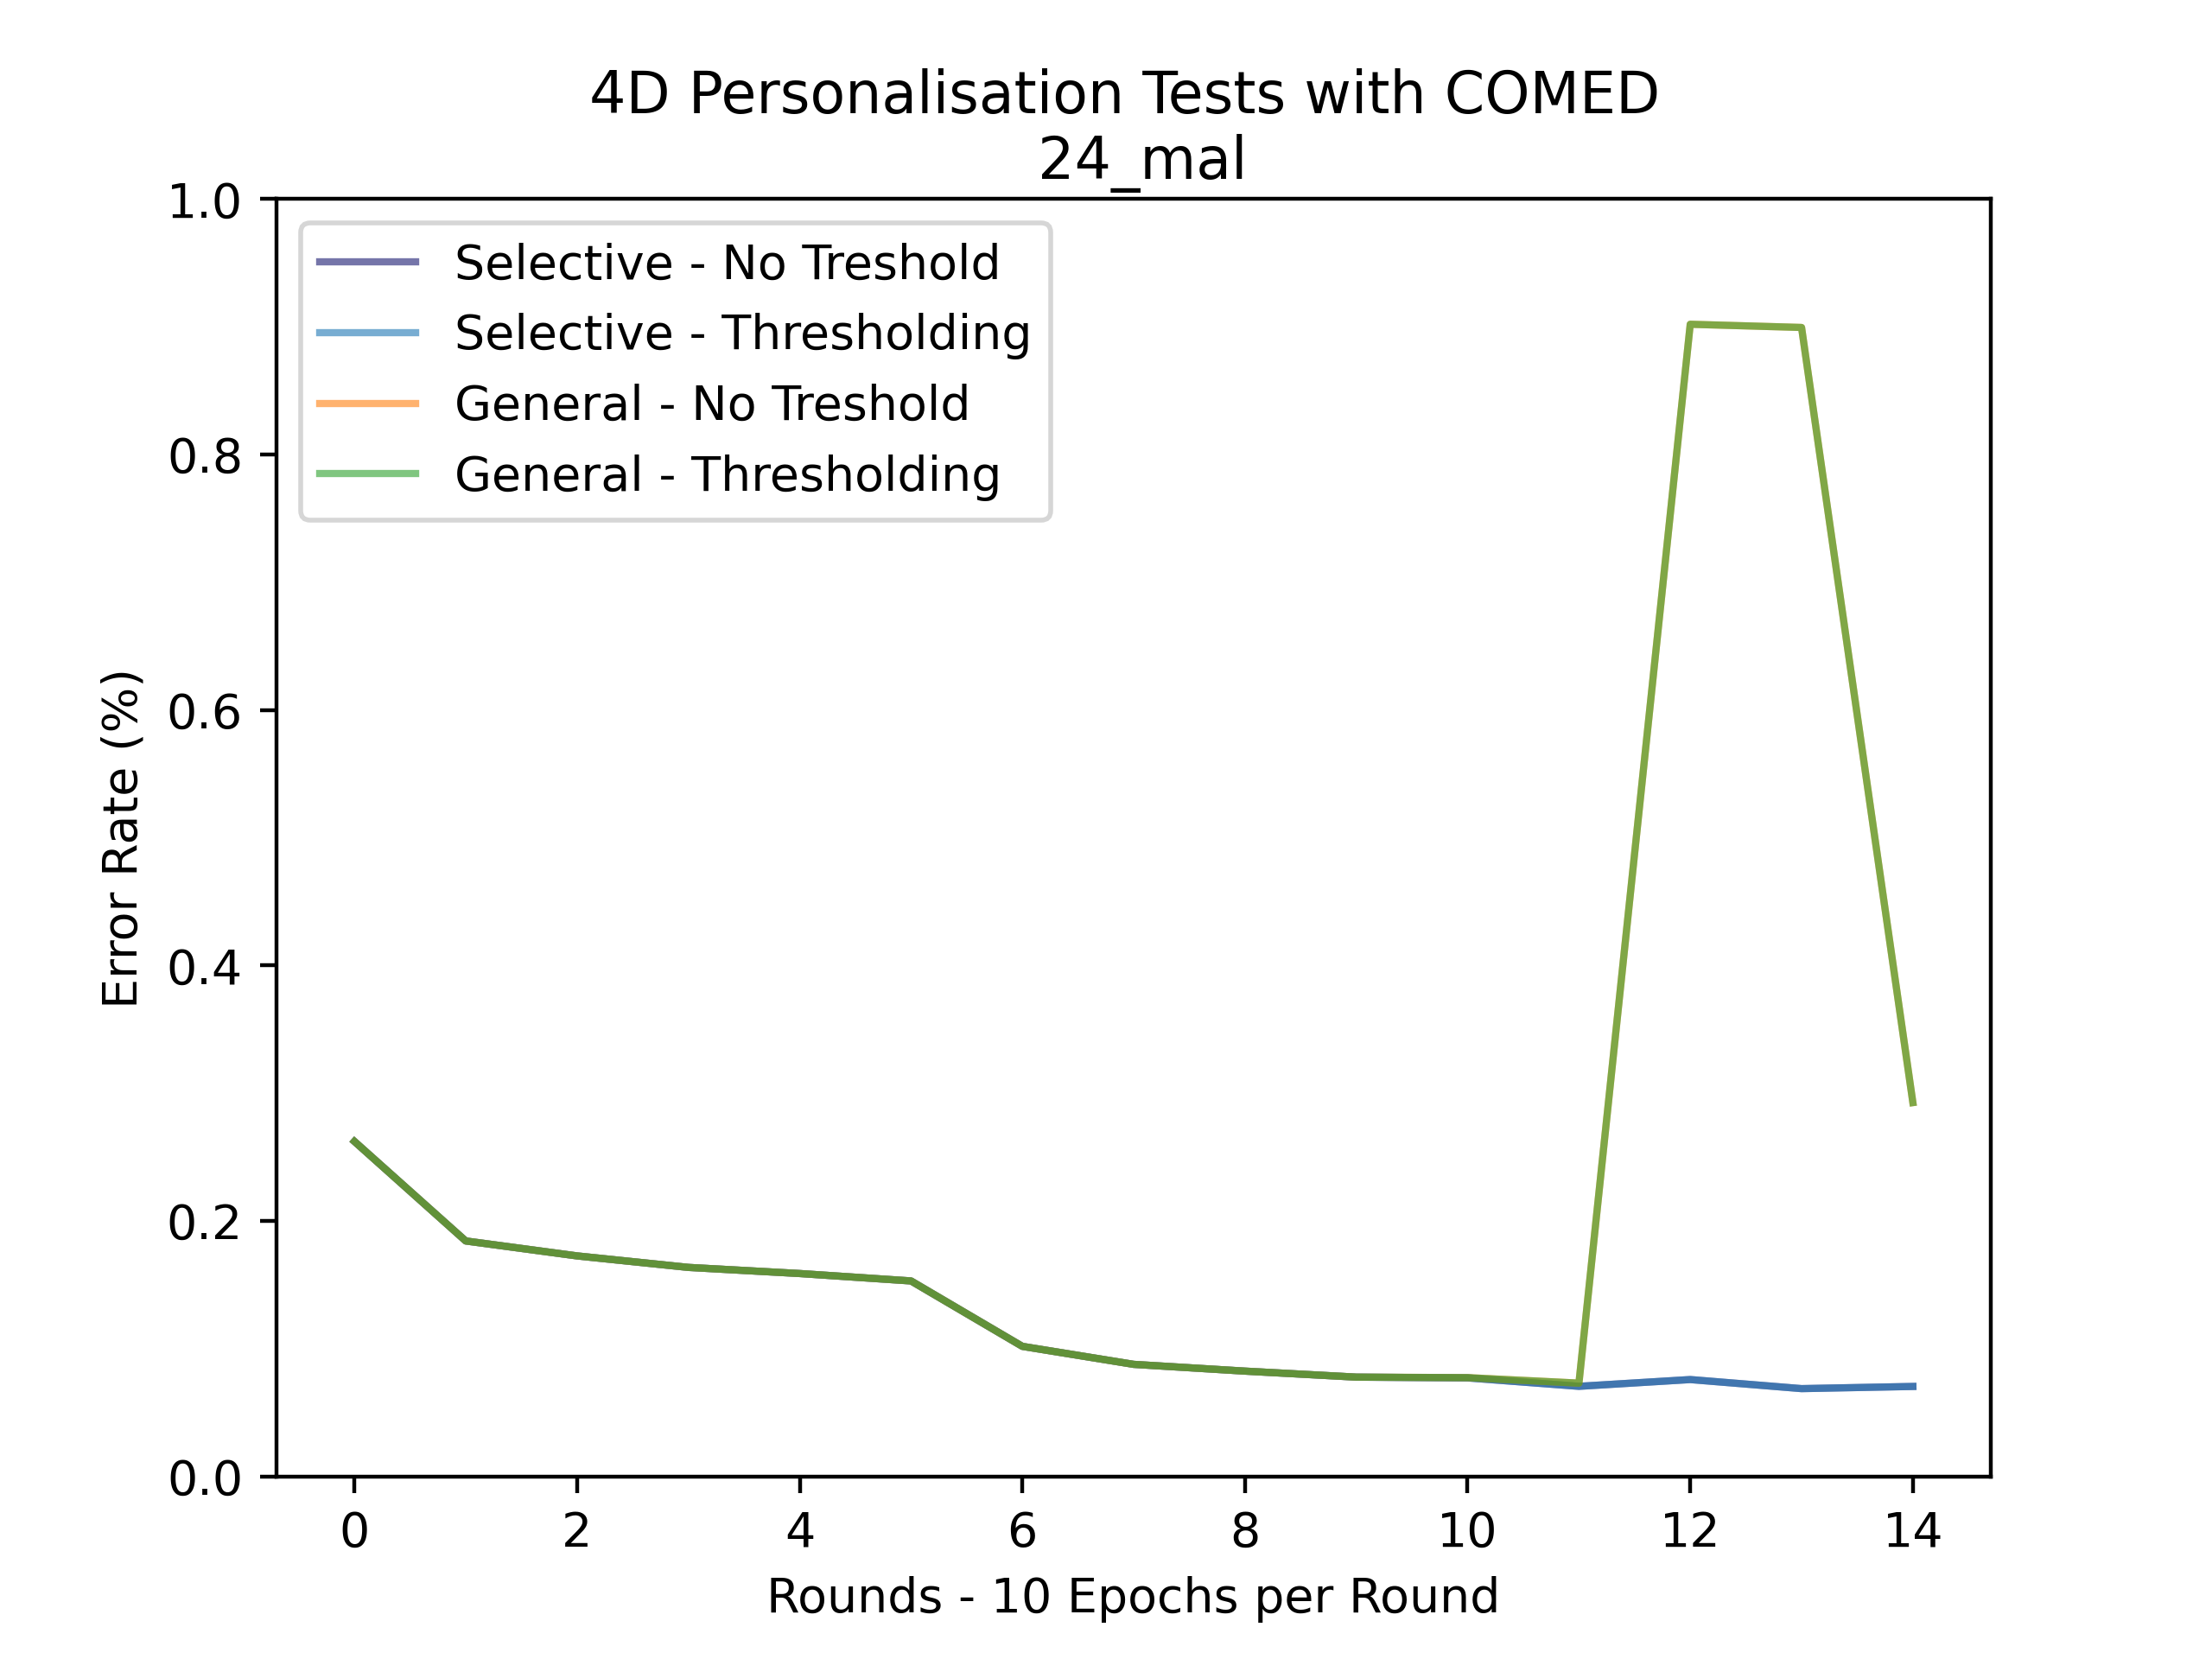
\includegraphics[scale=0.5]{my_agg/graphs/comed_4d_24mal.png}
	\caption{4D PCA with COMED as the External Aggregator under various Personalisation Methods - 24 Malicious}
	\label{fig:4d_24mal}
\end{figure}

\begin{figure}[htbp]
	\centering
    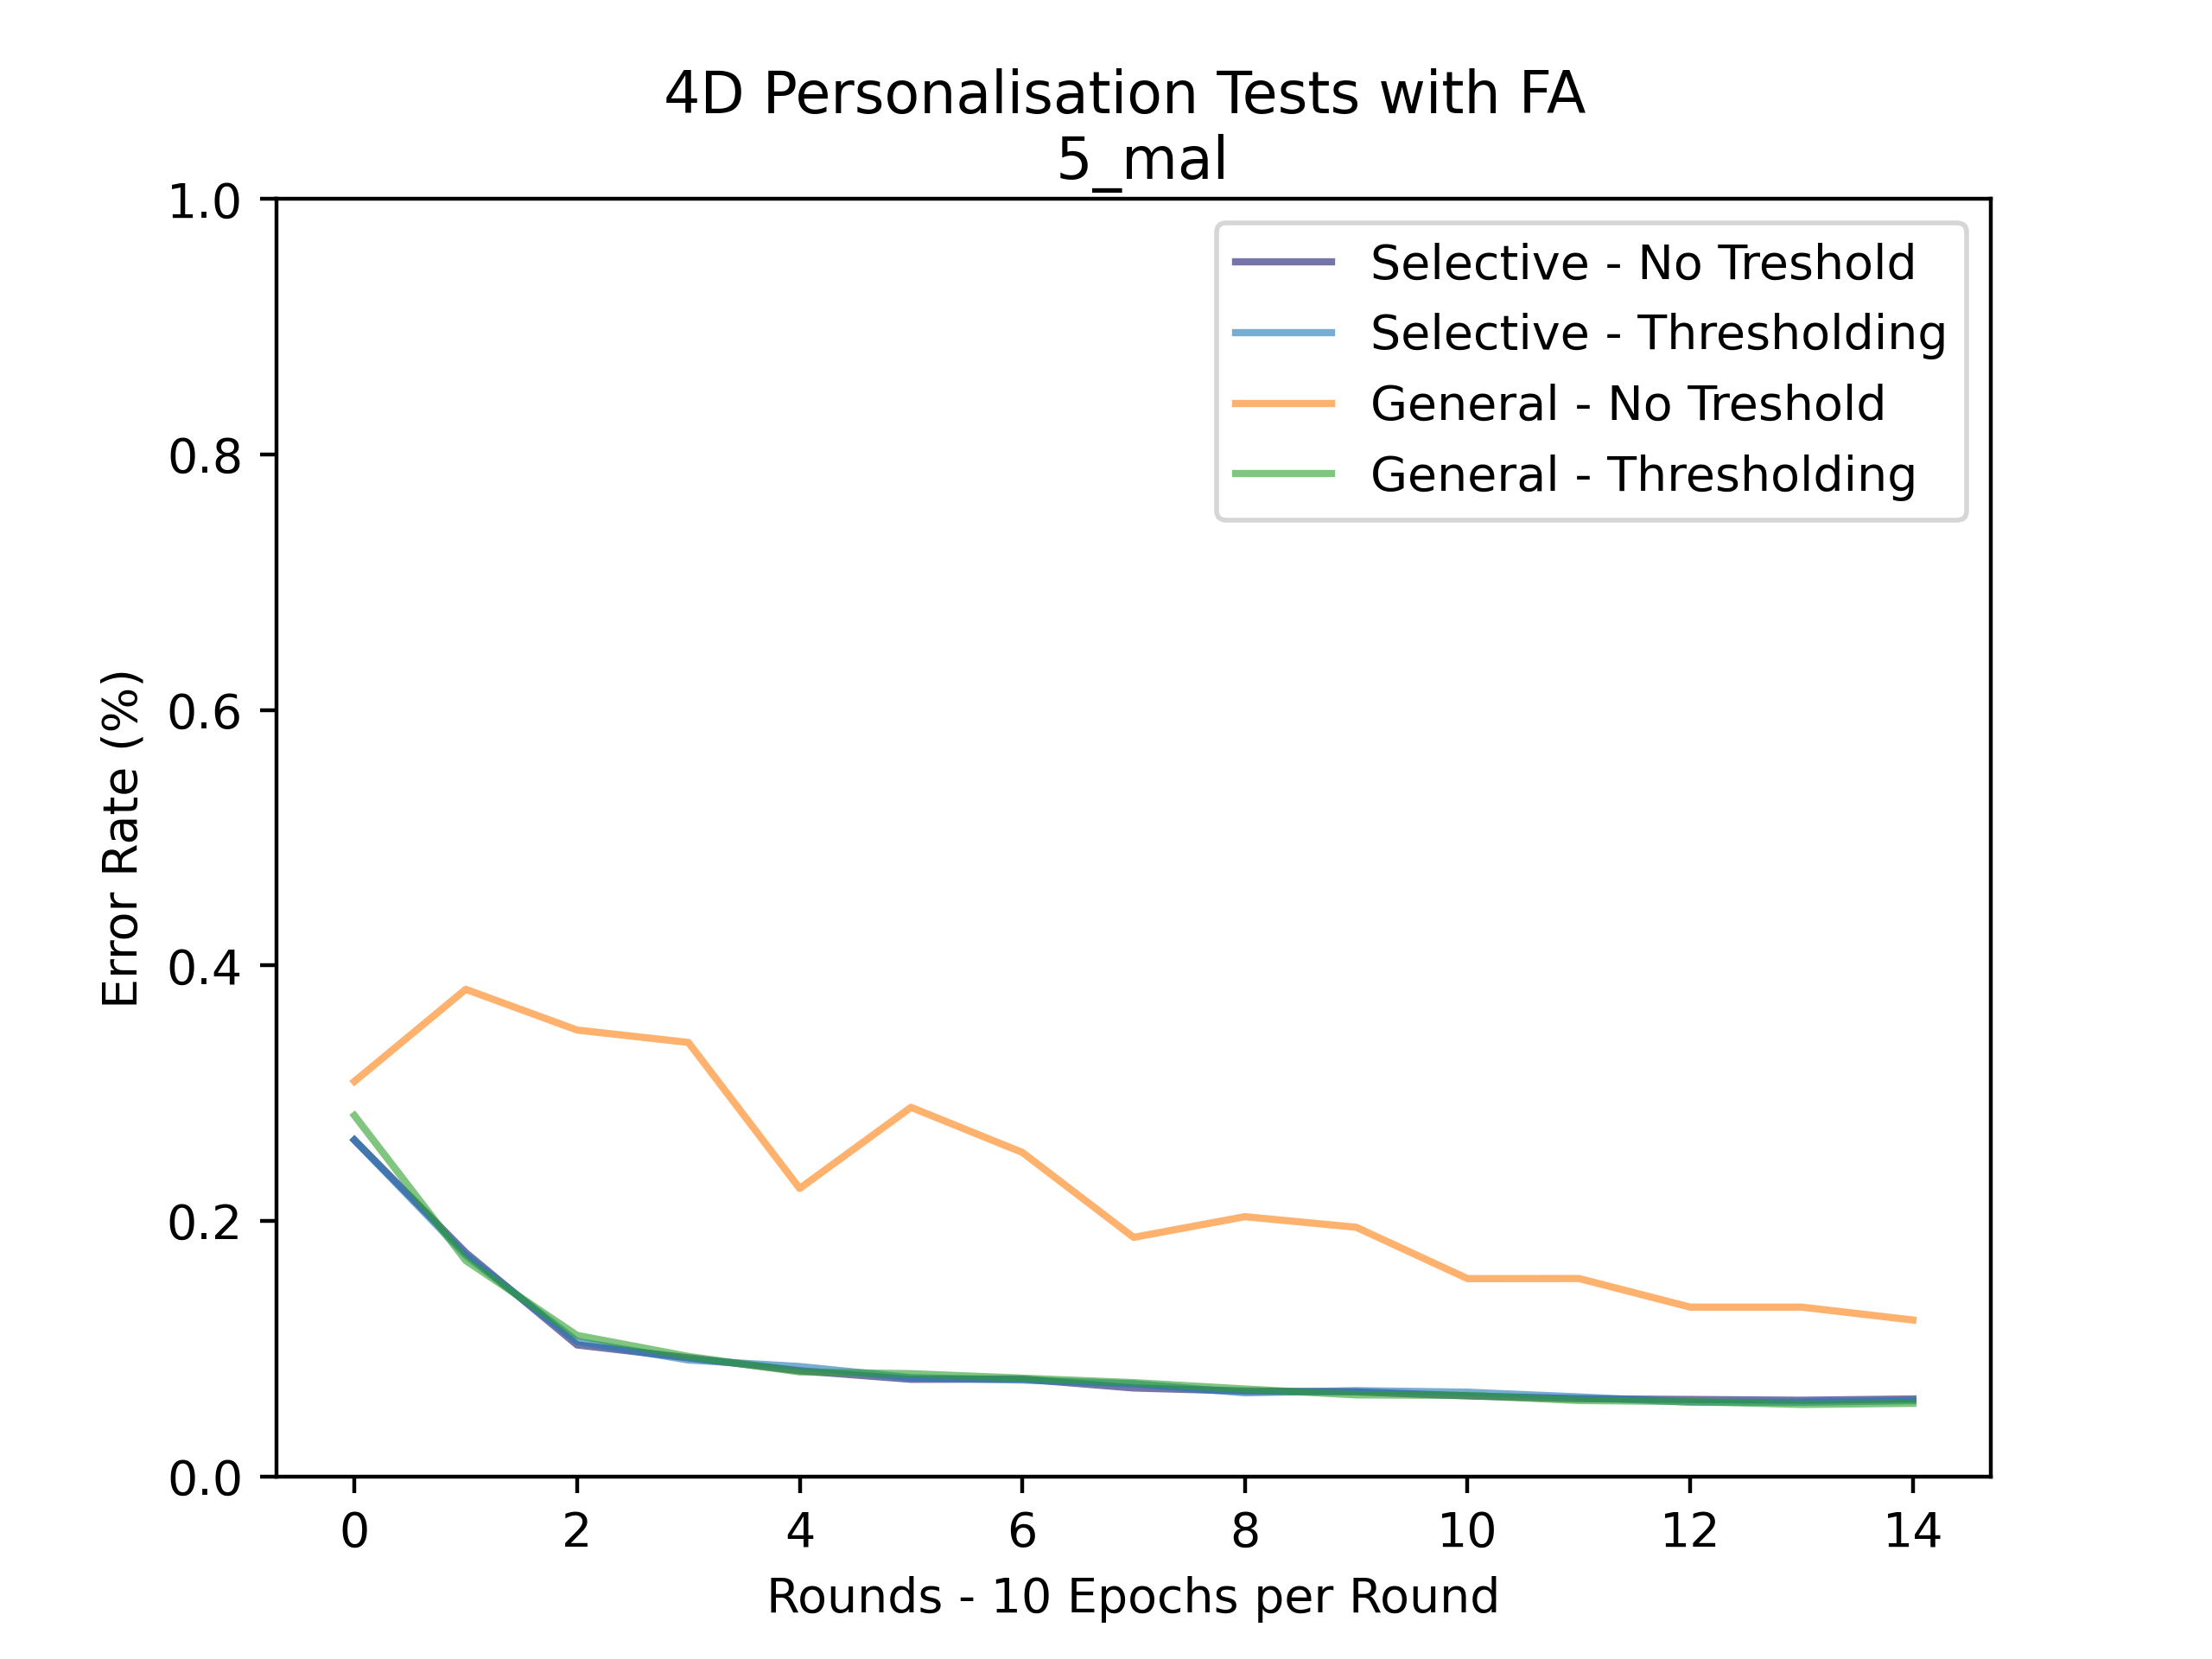
\includegraphics[scale=0.5]{my_agg/graphs/fa_4d_5mal.png}
	\caption{4D PCA with FedAvg as the External Aggregator under various Personalisation Methods - 5 Malicious}
	\label{fig:4d_5mal}
\end{figure}

\begin{figure}[htbp]
	\centering
    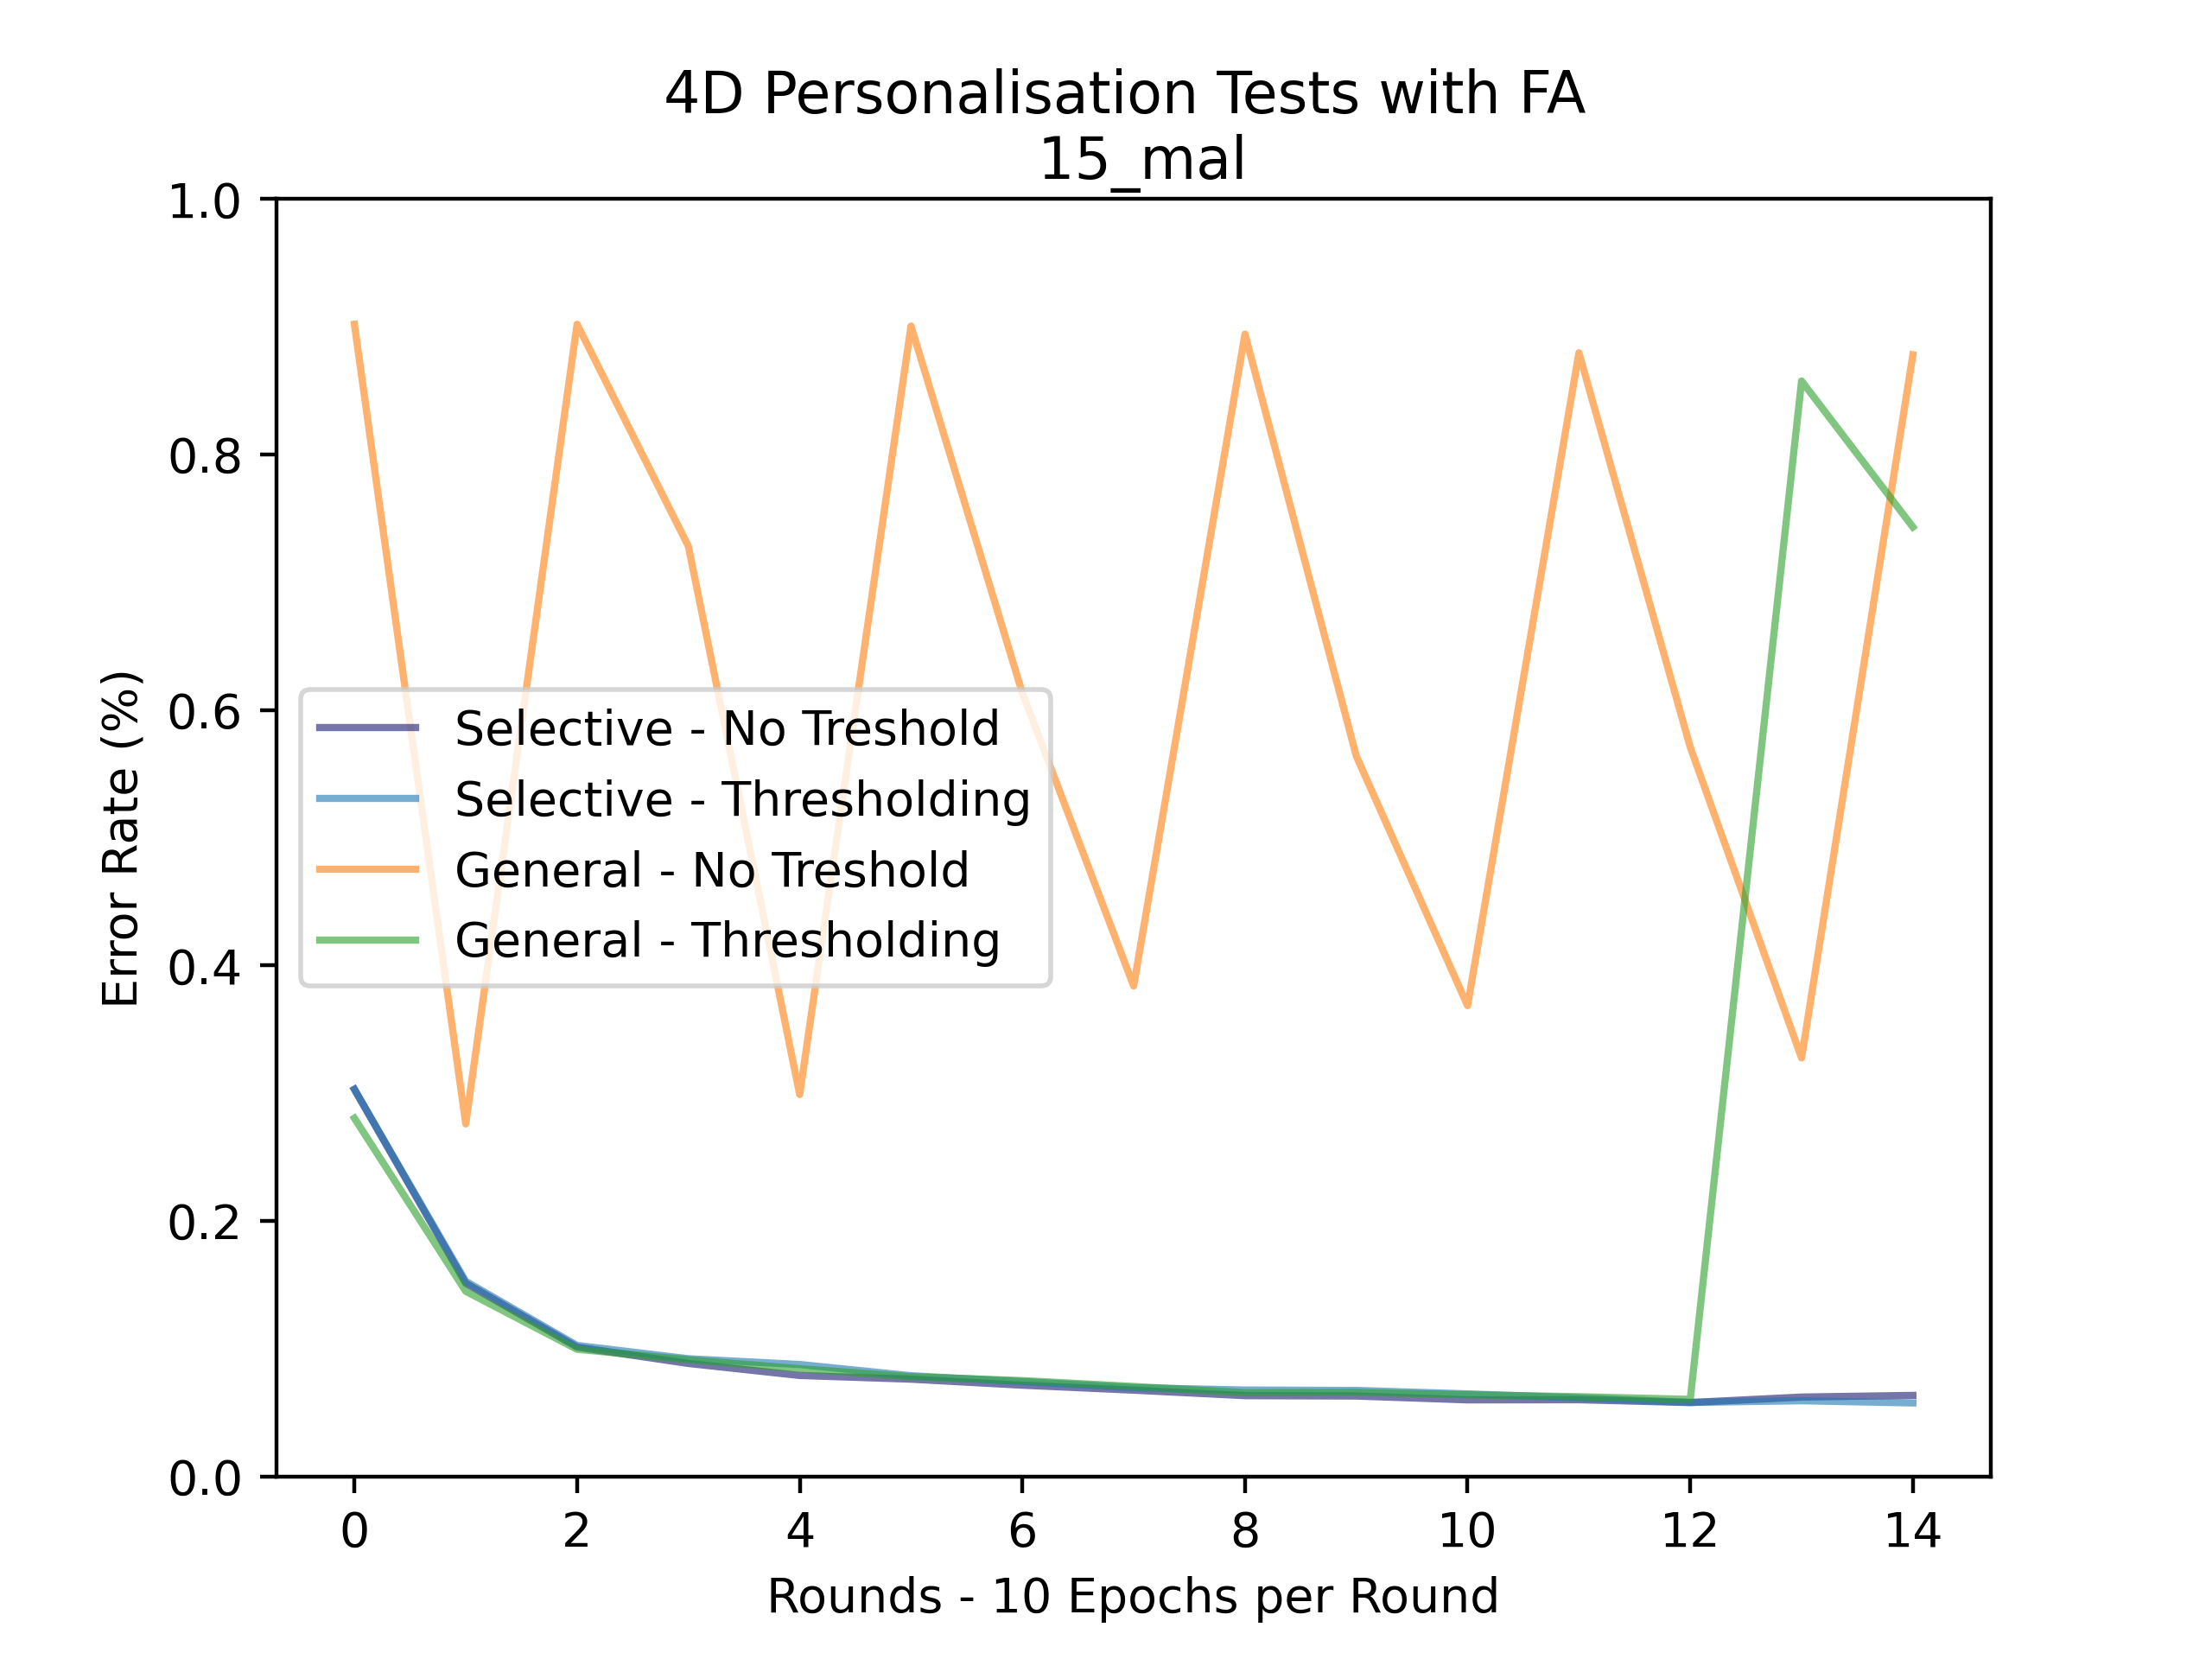
\includegraphics[scale=0.5]{my_agg/graphs/fa_4d_15mal.png}
	\caption{4D PCA with FedAvg as the External Aggregator under various Personalisation Methods - 15 Malicious}
	\label{fig:4d_15mal}
\end{figure}

\begin{figure}[htbp]
	\centering
    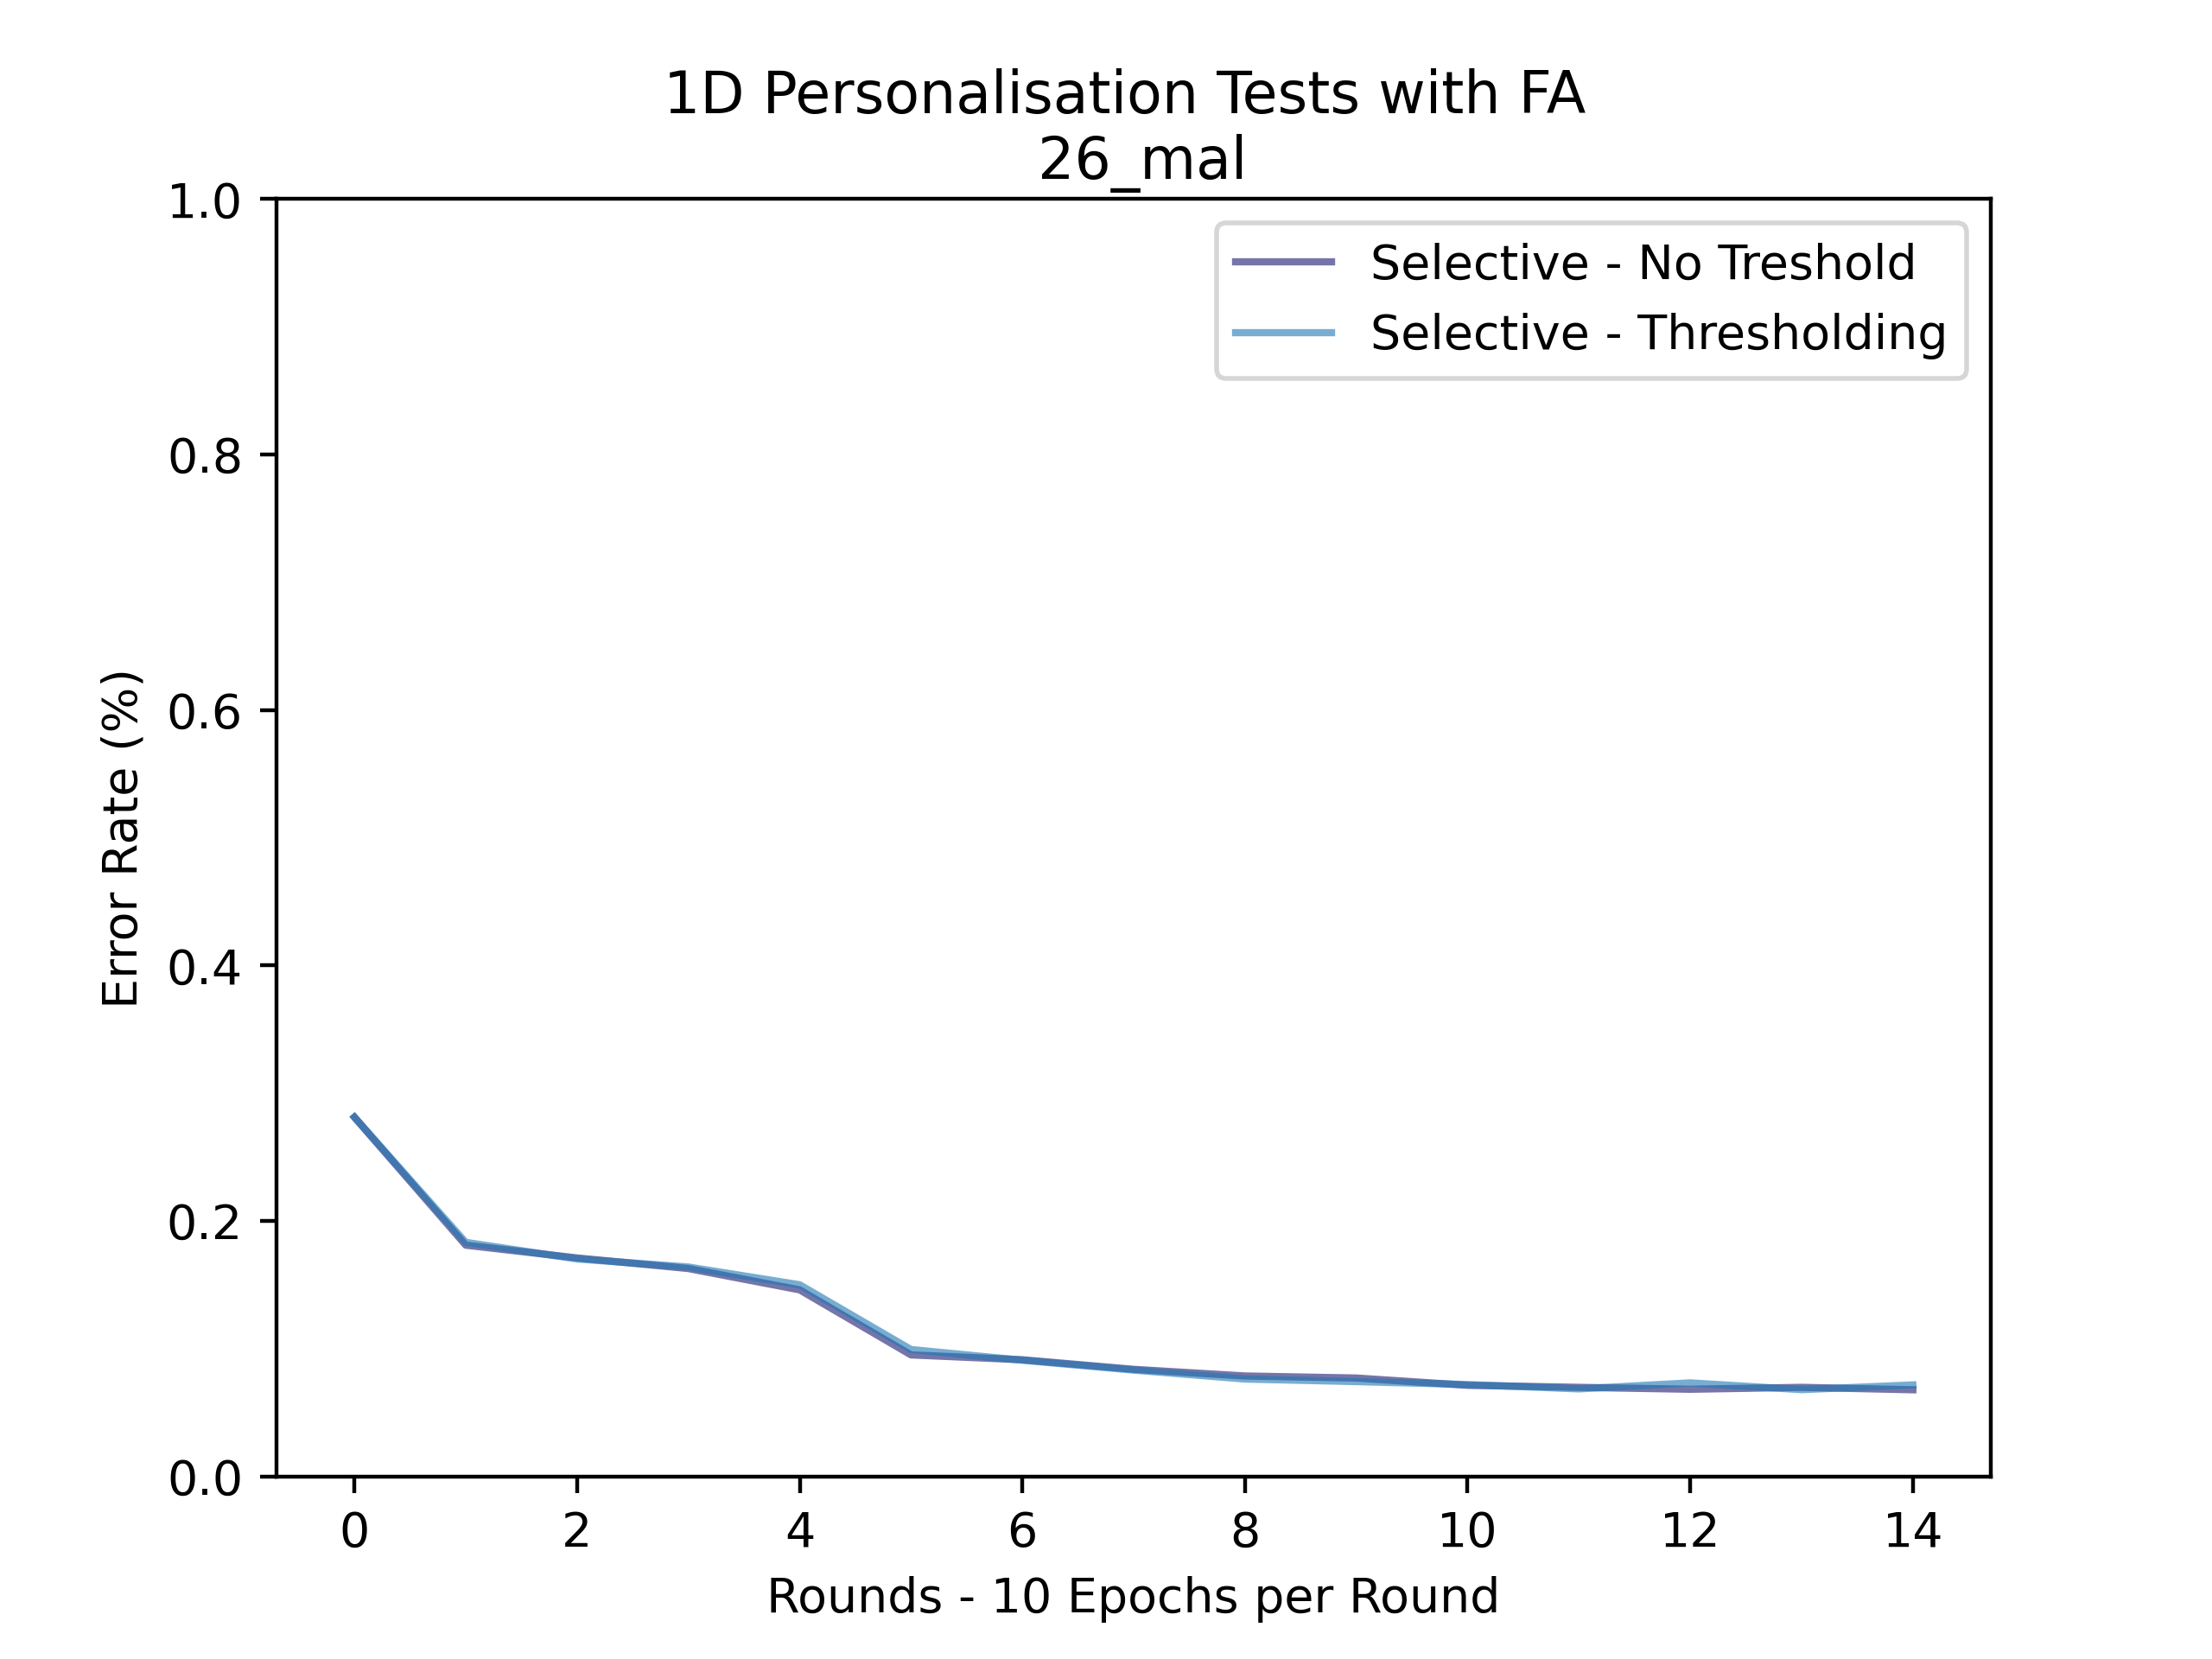
\includegraphics[scale=0.5]{my_agg/graphs/fa_1d_26mal.png}
	\caption{1D PCA with FedAvg as the External Aggregator under various Personalisation Methods - 26 Malicious}
	\label{fig:1d_26mal}
\end{figure}

\begin{figure}[htbp]
	\centering
    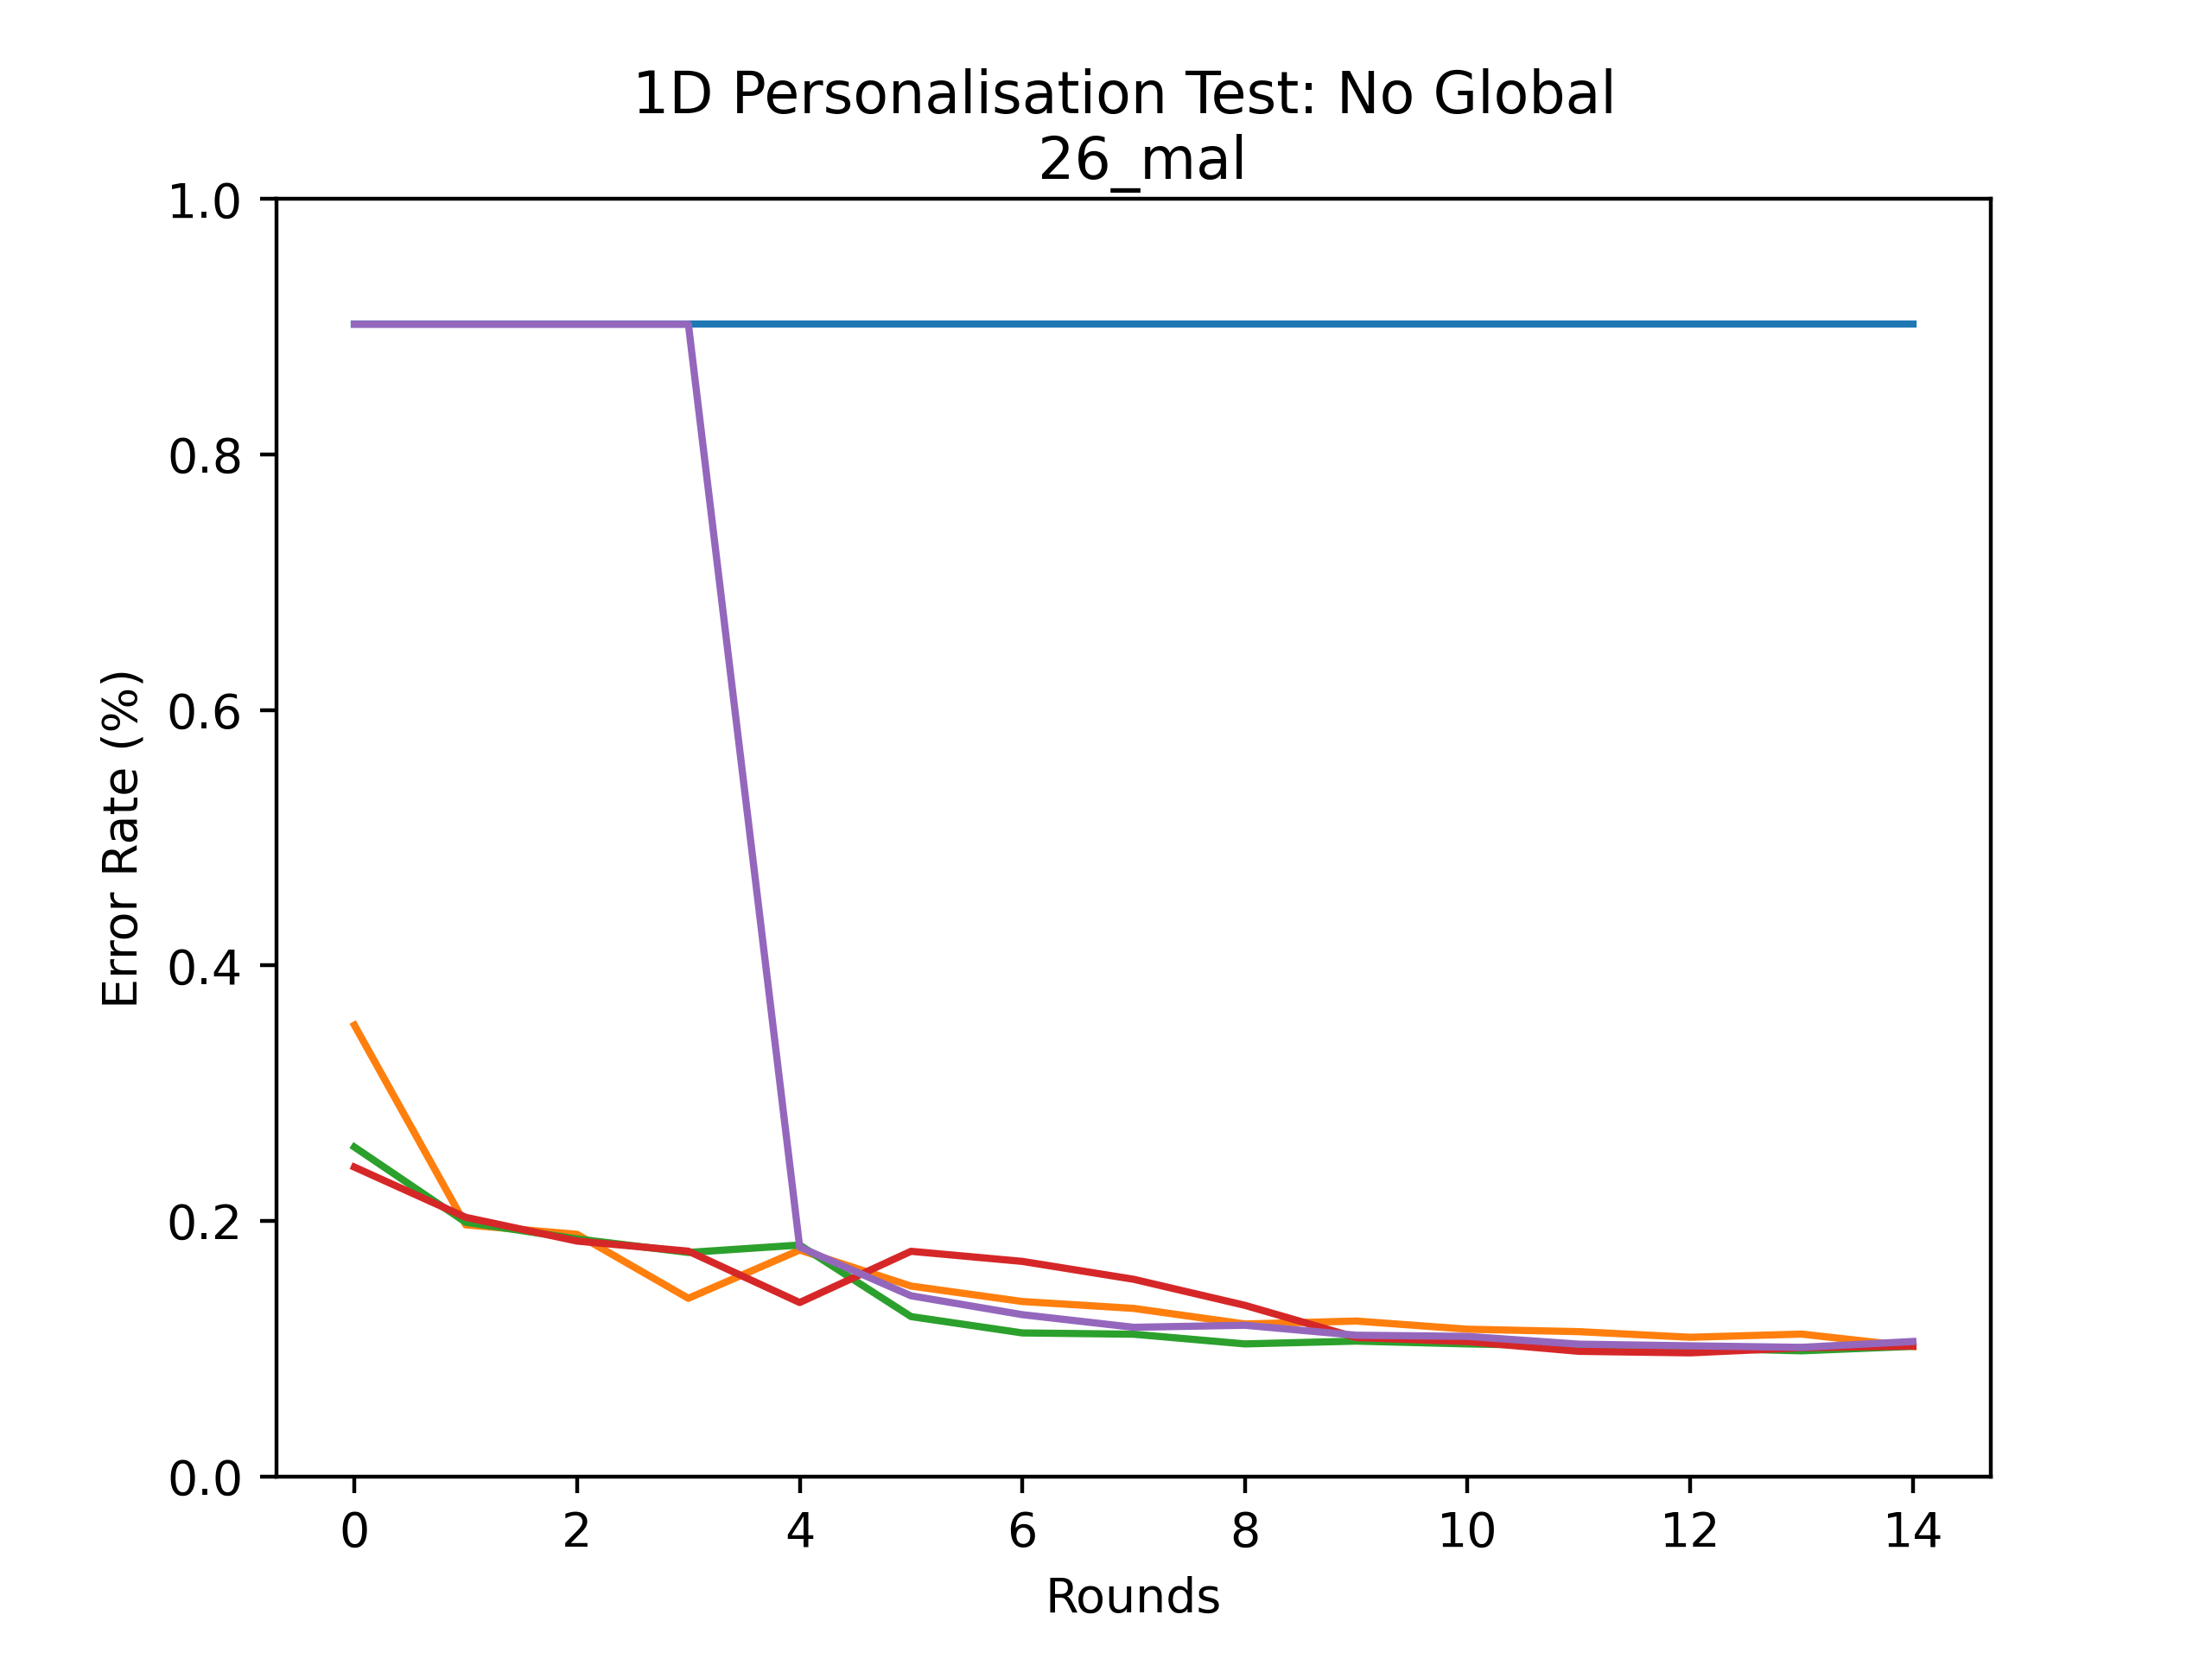
\includegraphics[scale=0.5]{my_agg/graphs/1d_no_global.png}
    \caption{4D PCA with the No Global Personalisation Method - 1 Malicious Client}
	\label{fig:4D_no_global_1}
\end{figure}

\begin{figure}[htbp]
	\centering
    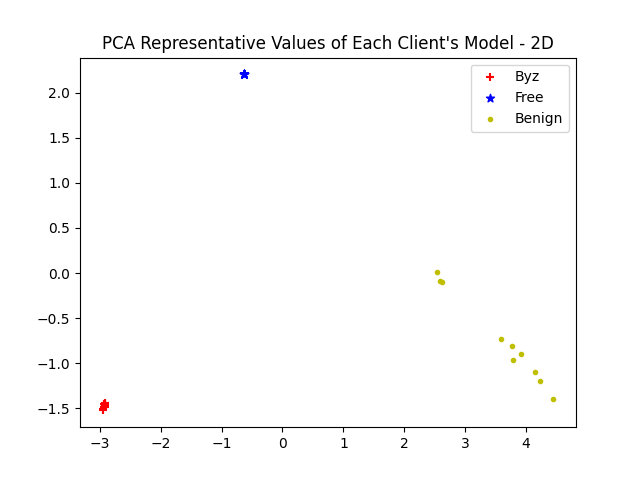
\includegraphics[scale=0.5]{my_agg/graphs/10mal_10free_r0_no_global.png}
    \caption{2D PCA Transform Representation with the No Global Personalisation Method - 10 Free, 10 Malicious at Round 0. This shows the separation of the clusters even when there are a combination of malicious and free-riding clients.}
	\label{fig:10mal10free_rep}
\end{figure}

\begin{figure}[htbp]
	\centering
    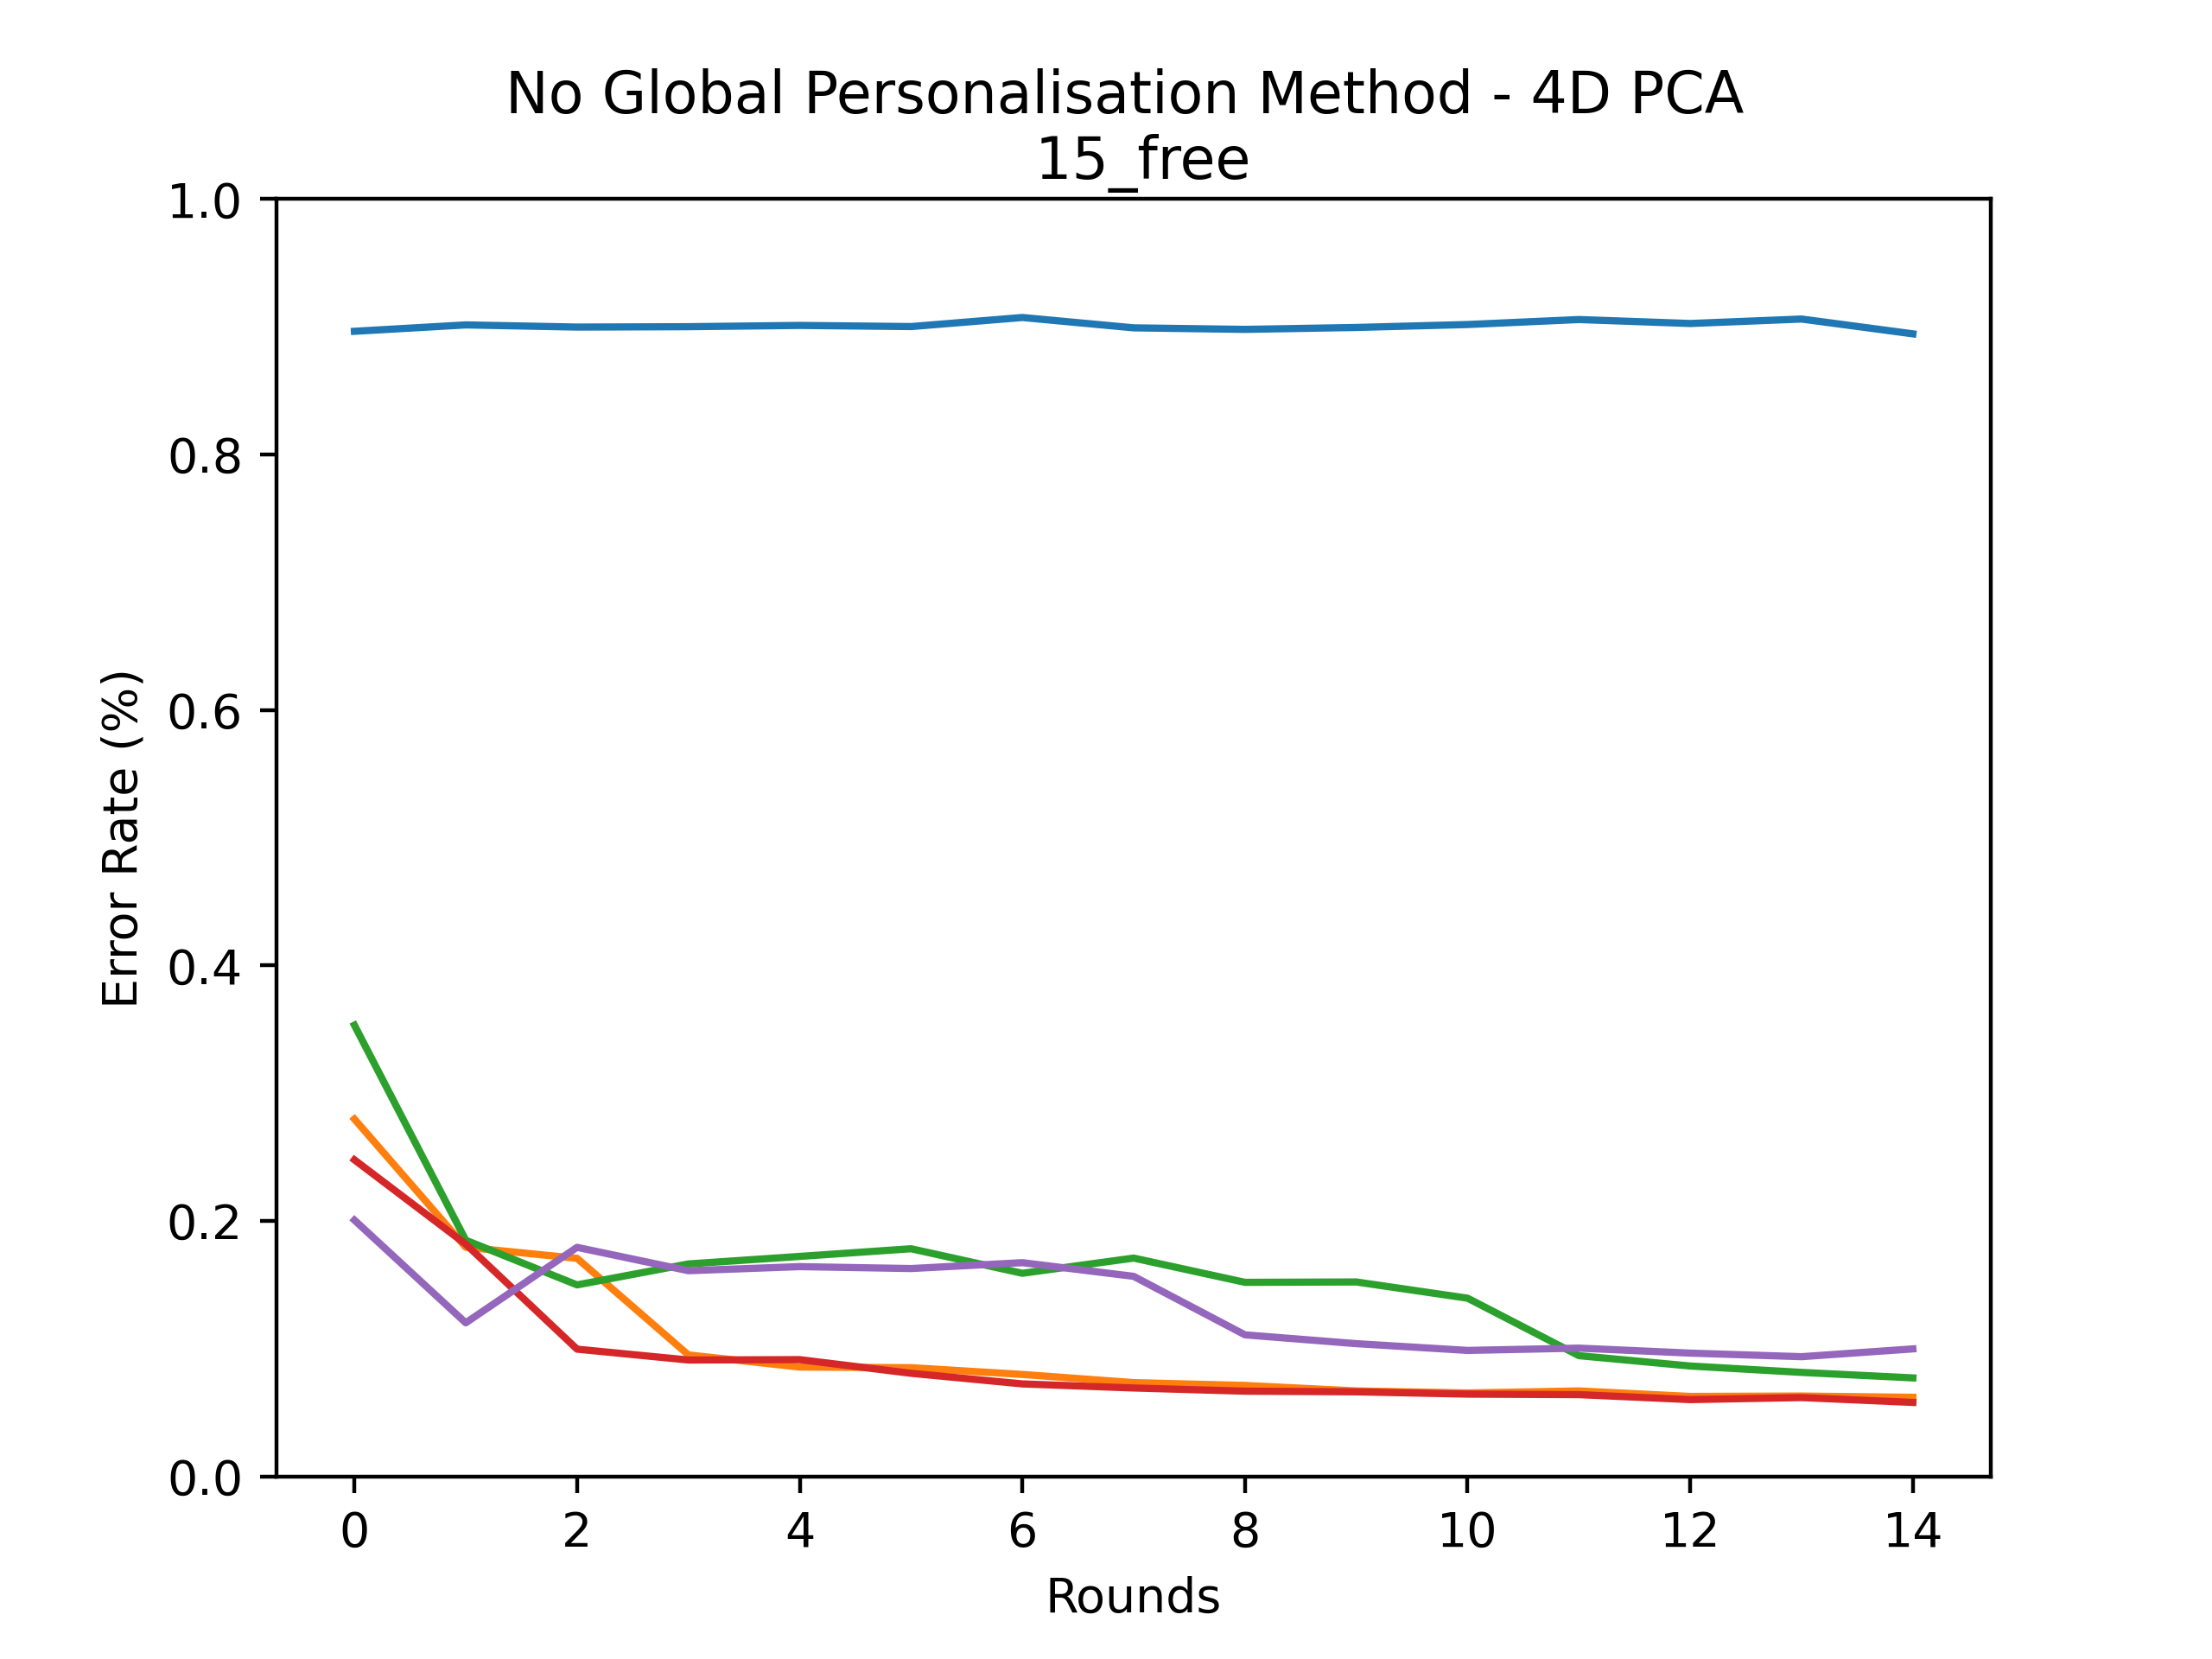
\includegraphics[scale=0.5]{my_agg/graphs/no_global_15free.png}
    \caption{4D PCA with the No Global Personalisation Method - 15 Free Clients. This shows Free-Riders not being able to ever learn as they are in the cluster represented by the top line.}
	\label{fig:no_15free}
\end{figure}
